%
% Template for Doctoral Theses at Uppsala 
% University. The template is based on    
% the layout and typography used for      
% dissertations in the Acta Universitatis 
% Upsaliensis series                      
% Ver 5.2 - 2012-08-08                  
% Latest version available at:            
%   http://ub.uu.se/thesistemplate            
%                                         
% Support: Wolmar Nyberg Akerstrom        
% Thesis Production           
% Uppsala University Library              
% avhandling@ub.uu.se                          
%                                         
%%%%%%%%%%%%%%%%%%%%%%%%%%%%%%%%%%%%%%%%%%%


\documentclass{UUThesisTemplate}

% Package to determine wether XeTeX is used
\usepackage{ifxetex}
\usepackage{mathtools}
\newcommand\isdef{\stackrel{\mathclap{\tiny\normalfont\mbox{def}}}{=}}
\ifxetex
	% XeTeX specific packages and settings
	% Language, diacritics and hyphenation
	\usepackage[babelshorthands]{polyglossia}
	\setmainlanguage{english}
	\setotherlanguages{swedish}

	% Font settings
	\setmainfont{Times New Roman}
	\setromanfont{Times New Roman}
	\setsansfont{Arial}
	\setmonofont{Courier New}
\else
	% Plain LaTeX specific packages and settings
	% Language, diacritics and hyphenation
    % Use English and Swedish languages. 
	\usepackage[swedish,english]{babel} 

	% Font settings
	\usepackage{type1cm}
	\usepackage[latin1]{inputenc}
	\usepackage[T1]{fontenc}
	\usepackage{mathptmx}
	
	% Enable scaling of images on import
	\usepackage{graphicx}
\fi


% Tables
\usepackage{booktabs}
\usepackage{tabularx}

% Document links and bookmarks
\usepackage{hyperref} 

% Numbering of headings down to the subsection level
\numberingdepth{subsection}

% Including headings down to the subsection level in contents
\contentsdepth{subsection}


% Uncomment to use a custom abstract dummy text
%\abstractdummy{
%	\begin{abstract}
%		Please use no more than 300 words and avoid mathematics or complex script.
%	\end{abstract}
%}


\begin{document}
\frontmatter
    % Creates the front matter (title page(s), abstract, list of papers)
    % for either a Comprehensive Summary or a Monograph.
    % Authors of Comprehensive Summaries use this front matter 
    \frontmatterCS 
    % Monograph authors use this front matter 
    %\frontmatterMonograph 
 
   % Optional dedication
   \dedication{Dedicated to our new Life: Emmanuel and Mathis}
 
    % Environment used to create a list of papers
    \begin{listofpapers}
    	\item Imaging single cells in a beam of live cyanobacteria. %\label{ImCell}
        \item Open dataset of live cyanobacterial cells imaged using an X-ray laser. %\label{DataCell}
        \item RedFlamingo: Suite for automated classification of diffraction patterns. %\label{RefFlamingo}
        \item Template-based classification of diffraction patterns. %\label{TempClass}
        \item Open dataset of RDV particles. %\label{DataRDV}
    \end{listofpapers}
    
    
    \begingroup
        % To adjust the indentation in your table of contents, uncomment and enter the widest numbers for each level
        %  E.g.  \settocnumwidth{widest chapter number}{widest section number}{widest subsection number}...{...}
       %  \settocnumwidth{5}{4}{5}{3}{3}{3}
        \tableofcontents
    \endgroup
    
    % Optional tables
    %\listoftables
    %\listoffigures

\mainmatter
    
    % Include your chapters here.
    %\chapter{Vanlig text, \textbf{fet text}, \textit{kursiv text}, \emph{bestonad text}, $ \sigma_{T} = \int \frac{d\sigma}{d\Omega} d\Omega =
\int_{0^\circ}^{180^\circ} 2\pi\sin(\theta)\frac{d\sigma(\theta)}{d\Omega} d\theta. $}

\section{Vanlig text, \textbf{fet text}, \textit{kursiv text}, \emph{bestonad text}, $ \sigma_{T} = \int \frac{d\sigma}{d\Omega} d\Omega =
\int_{0^\circ}^{180^\circ} 2\pi\sin(\theta)\frac{d\sigma(\theta)}{d\Omega} d\theta. $}

\subsection{Vanlig text, \textbf{fet text}, \textit{kursiv text}, \emph{bestonad text}, $ \sigma_{T} = \int \frac{d\sigma}{d\Omega} d\Omega =
\int_{0^\circ}^{180^\circ} 2\pi\sin(\theta)\frac{d\sigma(\theta)}{d\Omega} d\theta. $}

\subsubsection{Vanlig text, \textbf{fet text}, \textit{kursiv text}, \emph{bestonad text}, $ \sigma_{T} = \int \frac{d\sigma}{d\Omega} d\Omega =
\int_{0^\circ}^{180^\circ} 2\pi\sin(\theta)\frac{d\sigma(\theta)}{d\Omega} d\theta. $}

\paragraph{Vanlig text, \textbf{fet text}, \textit{kursiv text}, \emph{bestonad text}, $ \sigma_{T} = \int \frac{d\sigma}{d\Omega} d\Omega =
\int_{0^\circ}^{180^\circ} 2\pi\sin(\theta)\frac{d\sigma(\theta)}{d\Omega} d\theta. $}

\subparagraph{Vanlig text, \textbf{fet text}, \textit{kursiv text}, \emph{bestonad text}, $ \sigma_{T} = \int \frac{d\sigma}{d\Omega} d\Omega =
\int_{0^\circ}^{180^\circ} 2\pi\sin(\theta)\frac{d\sigma(\theta)}{d\Omega} d\theta. $}
Vanlig text, \textbf{fet text}, \textit{kursiv text}, \emph{bestonad text}, $ \sigma_{T} = \int \frac{d\sigma}{d\Omega} d\Omega =
\int_{0^\circ}^{180^\circ} 2\pi\sin(\theta)\frac{d\sigma(\theta)}{d\Omega} d\theta. $
Tester


\normalsize{Det h�r �r br�dtextstorlek i 11}

\tiny{Det h�r �r tiny i 6pt storlek}

\scriptsize{Det h�r �r scriptsize i 8pt storlek}

\footnotesize{Det h�r �r footnotesize i 9pt storlek}

\small{Det h�r �r small i 10pt storlek}

\large{Det h�r �r large i 13pt storlek}

\Large{Det h�r �r Large i 15pt storlek}

\LARGE{Det h�r �r LARGE i 18pt storlek}

\huge{Det h�r �r huge i 20pt storlek}

\Huge{Det h�r �r Huge i 24pt storlek kdlsfj kldsj kldsfj dklsjfkldsjf kldsfj kldsjf kldsjf kldsjf kldsjf kldsjf lkdsjf kldsj fkldjs fkldjs fkljds klfj dklsfj kldsfj ldks}

\normalsize

In Paper~\ref{pc} we show

    \part{Motivation}
\chapter{Motivation}
When a famous scientist was asked why he had a horseshoe hanging over his door he replied: "They say it works, whether you believe in it or not". The same can be said about science. Science attempts to build a framework of knowledge that transcends individual beliefs. Paradoxically the knowledge acquired through the scientific process relies on models and theories that are themselves simplifications of the phenomena they try to describe. Nonetheless, the power gained through the models and theories is enormous as for example antibiotics and acquired resistance through vaccination have extended and improved our lifetimes. Furthermore, by logical inference from existing models or theories new phenomena, phenomena that had never been observed before, might even be predicted. One such examples is the bending of the path of light by a heavy object like the sun. In this thesis I will try to show a few examples of how the field of science is evolving, how ideas themselves have evolved, and that many experiments are exploiting progress from many areas of science.

One field where I particularly feel attracted to is structural biology. Cellular life and the organization of its constituents are amazingly intricate and diverse. Proteins form an interconnected network of interactions in which temporal changes to individual proteins can trigger global responses such as the reshaping of macrophages in the presence of a bacterium or a cancerous cell[]. In order to understand the factors that activate or deactivate such pathways it is not enough to study individual components alone. A grand challenge of the 21st century is the imaging of \textit{live} cells, at atomic resolution, at a time resolution that allows capturing even the fastest biological processes.

Super resolution optical microscopy can image cells as a whole and has increased our understanding of cellular organization significantly. However the technique is ultimately limited by the size of the fluorescent label. X-ray crystallography can image large bio-particles at atomic resolution, but requires the particles to crystallize. For cells this is not possible. Nuclear Magnetic Resonance can study the dynamics of proteins at atomic resolution, at with nanosecond time resolution. Recently it has succeeded in studying labelled proteins \textit{in vivo} []. NMR is still limited by the size of the proteins it can study, as well as the collection time. It has been attempted to predict protein structure from backbone chemical shift only, which would avoid the must time consuming steps [Shen]. I have participated in the improvement of this method as shown in Paper V-X. This method works well for predicting the structure of ordered region.

The most promising method to study cells as well as its constituents at near-atomic resolution is cryo-electron microscopy. Focussed ion beams can be used to slice cryo-frozen cells into thin sections without considerably damaging them. This has solved the issue of penetration debt allowing the studying of internal features. Using sub-tomogram averaging, the structure of highly abundant proteins can be elucidated at resolutions beyond 4A []. For understanding rare events, however, acquisition time is a limiting factor. The time resolution of this field is currently limited to the microsecond range [].

A promising alternative that can be utilized to study living cells is femtosecond x-ray diffraction imaging (FXI). FXI uses the ultrashort and extremely bright pulses produced by free-electron x-ray lasers. The power of the pulse allows for single particle imaging (SPI). They femtosecond pulse outrun the key damage processes that occur due to the exposure to d
the beam. It is predicted that sub-nanometer resolution can be achieved on micron-sized cells  \cite{Bergh2008}. The femtosecond pulse gives an unprecedented time resolution that captures any biologically relevant motion, all at room temperature. Another big advantage of this method is the repetition rate. The recently operational EuXFEL can have repetition rates of 27000 Hz, potentially allowing the recording of over a billion images a day. This might enable the imaging of rare cellular events.

This thesis deals with the experimental verification of FXI on living cells, and studies if, and what, computational and experimental tools are necessary to make cell imaging a reality. It will start by explaining the general framework necessary for each step of the experiment: The generation of X-rays, sample introduction, the interaction of light and matter, the recording of two-dimensional (2D) diffraction pattern, the reconstruction of cell images, how 2D images might be combined to derive three-dimensional (3D) structural information, and finally how image classification might be useful for the latter two. The final chapters describe the results on life cell imaging, and how image classification has been used for imaging reconstruction and pattern selection.




    \part{Concept}%

\chapter{Interaction of Light and Matter}
Traditionally cells have been studied with optical light. To understand why light is a good probe to study cells, it is necessary to understand the nature of its interaction with matter. For most work described in this thesis the classical model of describing light as a wave is sufficient. This chapter will create the mathematical framework that describes how light behaves in our diffraction experiments. 

\section{Light as electromagnetic radiation}
In the 17th and 18th century it became possible for humans to generate electric charges and continuous currents [Guericke, Leiden, Volta], enabling the investigation of the phenomena of electricity and magnetism. This ultimately led to a ground-breaking work by Maxwel where he ties together the fields of magnetism, electricity, and somewhat surprisingly, optics. His results are known as the Maxwell equations:

\begin{equation} \nabla \cdot   \vec{E} = \frac{\rho}{\varepsilon_0 }\label{eq:maxlaw1}\end{equation}
\begin{equation} \nabla \cdot   \vec{B} = 0 \label{eq:maxlaw2}\end{equation}
\begin{equation} \nabla \times \vec{E} = -\frac{d\vec{B}}{dt}\label{eq:maxlaw3}\end{equation}
\begin{equation} \nabla \times \vec{B} = \mu_0 \vec{J} -\mu\varepsilon\frac{d\vec{E}}{dt}\label{eq:maxlaw4}\end{equation}

Here, $\vec{E}$ is the electric field, $\vec{B}$ is the magnetic field, $\varepsilon$ and $\mu$ are respectively the permittivity and the permeability of the material. $\rho$ is the the charge density and $\vec{J}$ describes the local current. %Equation \ref{eq:maxlaw1} shows that the electric flux
%leaving a volume is proportional to the charge inside. Equation
%\ref{eq:maxlaw2} states that the magnetic flux leaving a volume is
%always 0. This means that the north and south pole of a magnet are
%always connected, which finds its origin in the dipole moment of the
%electron itself. Equation \ref{eq:maxlaw3} shows that the voltage
%induced in a closed loop in proportional to the rate of change of the
%magnetic flux that the loop encloses. A dynamo uses this phenomena to
%generate a charge. Equation \ref{eq:maxlaw4} shows that the magnetic
%field induced around a closed loop is proportional to the electric
%current plus the rate of change in the electric field. Electric motors
%exploit this phenomena. 
An important consequence of these equations is that a moving charge will induce a magnetic field, which in its turn induces a change in the electric field, and so on.

In order to understand why these laws unify magnetism, electricity and optics, we will consider a special case: vacuum. In vacuum there are no localized charges ($\rho = 0$) and no currents ($\vec{J}=0$), which simplifies equation \ref{eq:maxlaw1} and \ref{eq:maxlaw4} to: 

\begin{equation} \nabla \cdot   \vec{E} = 0 \label{eq:maxlaw1_vac}\end{equation}
\begin{equation} \nabla \times \vec{B} = -\mu_0\varepsilon_0\frac{d\vec{E}}{dt}\label{eq:maxlaw4_vac}\end{equation}

Furthermore, experiments showed that the permittivity for vacuum, $\varepsilon_0 = 8.854\cdot10^{-12} Fm^{-1}$, and the permeability for vacuum$mu_0 = 1.257 \cdot 10^{-7} N A^{-2}$. If we now ask ourselves what the field change caused by a change in the electric field is by studying the equation $\nabla \times( \nabla \times \vec{E}) $, we can derive something quite amazing:  
\[ \nabla \times( \nabla \times \vec{E}) = \nabla (\nabla \cdot
\vec{E}) -\nabla^2 \vec{E} =-\nabla^2 \vec{E} \]
The first equality is a well known mathematical relation, and for the second equality equation \ref{eq:maxlaw1_vac} is used. 
Now lets rewrite the equation in a different way:
\[\nabla \times( \nabla \times \vec{E})=
\nabla\times(-\frac{d\vec{B}}{dt}) =
-\frac{d}{dt}(\nabla\times\vec{B})=\frac{d}{dt}(\mu_0\varepsilon_0\frac{d\vec{E}}{dt})
= \mu_0\varepsilon_0\frac{d^2\vec{E}}{dt^2}\]
In the first equality we used equation \ref{eq:maxlaw3}. In the second equality we used a general algebraic property. In the third equality we used \ref{eq:maxlaw4_vac}, and in the last equality we combined the two time derivatives. Together these equations state that:

\begin{equation}\label{eq:wave_eq}
\frac{d^2\vec{E}}{dt^2} = \frac{1}{\mu_0\varepsilon_0}\nabla^2 \vec{E} = v^2 \nabla^2 \vec{E},      v = \frac{1}{\sqrt{\mu_0\varepsilon_0}}
\end{equation}

Equation \ref{eq:wave_eq} is known as the wave equation, which is used to describe the propagation of a wave with the speed $v$. Combining this results with the experimentally determined value for $\mu_0$ and $\varepsilon_0$ shows that electromagnetic (EM) waves travel at \(3\cdot 10^8 \frac{m}{s}\), which agreed with value of the speed of light \cite{Froome1971}. This result strongly hints at the possibility that light is an electromagnetic wave. Further experiments succeeded in demonstrating the existence of electromagnetic waves with long wavelengths and showed that their properties are consistent with the properties of visible light, including their velocity. Visible light has now become part of the broader spectrum of electromagnetic radiation. Although Quantum Mechanics complicated the description of light further, as light demonstrates particle-like behaviour under certain conditions. Many phenomena however can be described by treating light as a wave. 

\section{Photon-material interactions}
Assuming that light is electromagnetic radiation, it is easy to understand that a change in electric field will affect its propagation. There are four mechanisms through which radiation interacts with matter: photoabsorption, scattering, photo-nuclear absorption and pair production. The description of these phenomena will treat as if light will come in discrete quanta: photons. 
Photonuclear absorption and pair production only occur when matter is exposed to high energy gamma rays, and are therefore of little relevance to this thesis. Photoabsorption is facilitated primarily through a process called photoexcitation, in which an electron is excited to a higher level of energy, or possibly ionized in the case of photoionisation. Scattering can be divided into two classes: elastic scattering and inelastic scattering. Elastic scattering does not result in a change of kinetic energy of the scattering particle, nor does it change the wavelength of the radiation. Only the direction of the radiation can be changed. Inelastic scattering leads to both a change in wavelength of the radiation, and a change in kinetic energy. Photo-absorption and inelastic scattering deposit energy into the object which will lead to structural changes of the object. Elastic scattering on the other hand can be used to gain structural information about the object, without causing damage to the object. 

\section{Scattering by a single free electron}
The simplest example of elastic scattering is Thompson scattering from a free electron. A free electron will scatter or diffract the incoming radiation in all directions. An important physical concept for understanding scattering on a deeper level is the Lorentz force which describes the force exerted on a charged particle travelling in a electromagnetic field. 
\begin{equation}\label{eq:lorentz}
\vec{F} = q\vec{E} + q\vec{v}\times\vec{B}
\end{equation} 

From Newton's second law of motion ($\vec{F} = m \vec{a}$) it is known that force and acceleration are
proportional and parallel, thus the Lorentz force describes the acceleration of a charge in an electric and/or magnetic field. The first term of equation \ref{eq:lorentz} is also known as the Coulombic force, and shows that a charge is accelerated in the direction of an electric field. The second term shows that a moving charge is accelerated by the presence of a magnetic field in the direction that is both perpendicular to its movement and the magnetic field, given that $\vec{v}$ and $\vec{B}$ are not parallel in which case there is no acceleration.

According to classical electromagnetic theory the electric field associated with a monochromatic plane wave of amplitude $E_0$, and wavelength $\lambda$, propagating in the z-direction can be described by: 

\begin{equation}\label{eq:plane_wave}
\vec{E_{in}} = E_0 e^{-2\,\pi\ i \frac{ c t }{\lambda}}
\end{equation} 

When the oscillating electric field of the incident EM wave hits a stationary electron of mass $m_e$ and charge $e$ located at position $z = 0$, it exerts a Coulombic force on the electron which causes it to oscillate at the same frequency as the incident radiation. By Newton's second law of motion:

\begin{align}\label{eq:motion_single}
\vec{F} = m_e \vec{a}(t) =& e E_0 e^{-2\,\pi\ i \frac{ c t}{\lambda}} \\
\vec{a}(t) =& \frac{e\,E_0}{m} e^{-2\,\pi\ i \frac{c\,t}{\lambda}}
\end{align}

Here we assumed the contribution of the magnetic part of field to be negligible, as the electron will not reach a significant velocity.
An accelerated charge emits electromagnetic radiation. The oscillating electron becomes a new source of radiation that radiates spherically in all directions, at the same frequency as the incident radiation. From Maxwell's equations it follows that the electric field generated by an accelerating electron measured at point $\vec{d}$  can be described as []:

\begin{equation}\label{eq:scattering}
\vec{E_s}(\vec{d},t) = \frac{e a_\perp(t)}{4 \pi \varepsilon_0c^2d}
\end{equation}

$a_{\perp}(t)$ is the acceleration projected on a plane perpendicular to $\vec{d}$. 
\begin{equation}\label{eq:acceleration_perpendicular}
a_\perp = |\vec{a(t)}|\sin(\theta)
\end{equation}

Combining equations \ref{eq:motion_single}, \ref{eq:scattering}, and \ref{eq:acceleration_perpendicular}, we get that the instantaneous scattered field is:
\begin{equation}
E_s(\vec{d},t) = \frac{{e}^2}{4 \pi \varepsilon_0 m_e\,c^2} \frac{E_0 \sin(\theta)}{d} e^{-2\,\pi\ i \frac{|\vec{d}|}{\lambda}}
\end{equation}

The classical electron radius $r_e$ can be used to simplify the equation for the scattered field $E_s$
\begin{align*}
E_s=& - \frac{r_e\,E_0\,\sin(\theta)}{d} e^{-2\,\pi\ i \frac{|\vec{d}|}{\lambda}}\\
r_e =& \frac{e^2}{4 \pi \varepsilon_0 m_e\,c^2}    
\end{align*}


\section{Two-body scattering}
%\subsection{Approximations} 
If more than one electron are present the scattered waves will interfere, similar to the interference of water waves. The resulting pattern of dark and light bands is called a diffraction pattern. The first person to report this phenomenon was Grimaldi in 1660. Whether the interference is constructive of destructive depends on the optical path difference (OPD) between the scattered waves. Waves with path differences close to integer numbers of wavelengths interfere constructively, if close to half integral waves will interfere destructively. The central light band is often referred to as the zeroth diffraction order, or more colloquially as the central speckle. The light band next to it is called the first diffraction order (or first fringe), the one next to that the second order and so on. These terms will be used throughout the thesis. Figure \ref{fig:Interference} illustrates the phenomenon of interference.

\begin{figure}[h]
\centering 
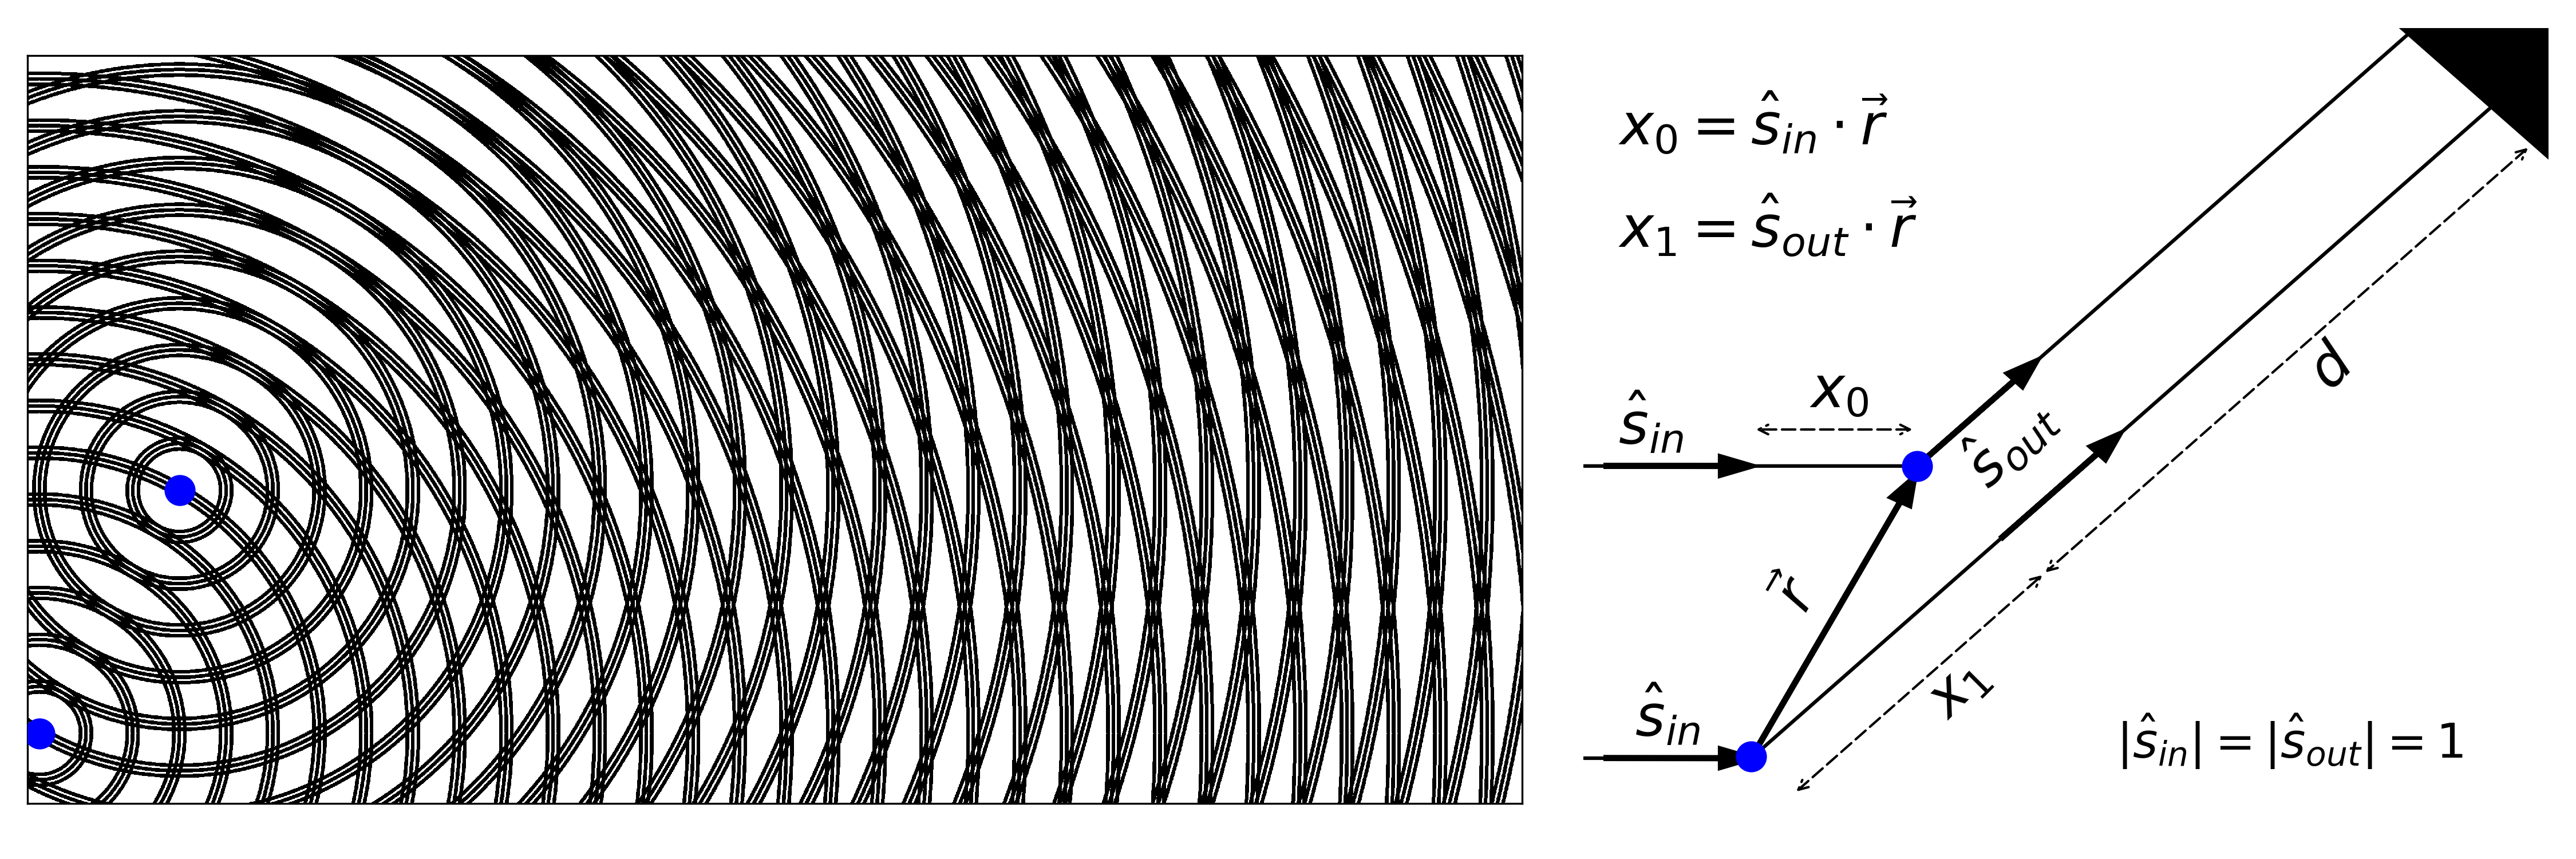
\includegraphics[width=120mm]{InterferenceTwoElectrons3.png}
%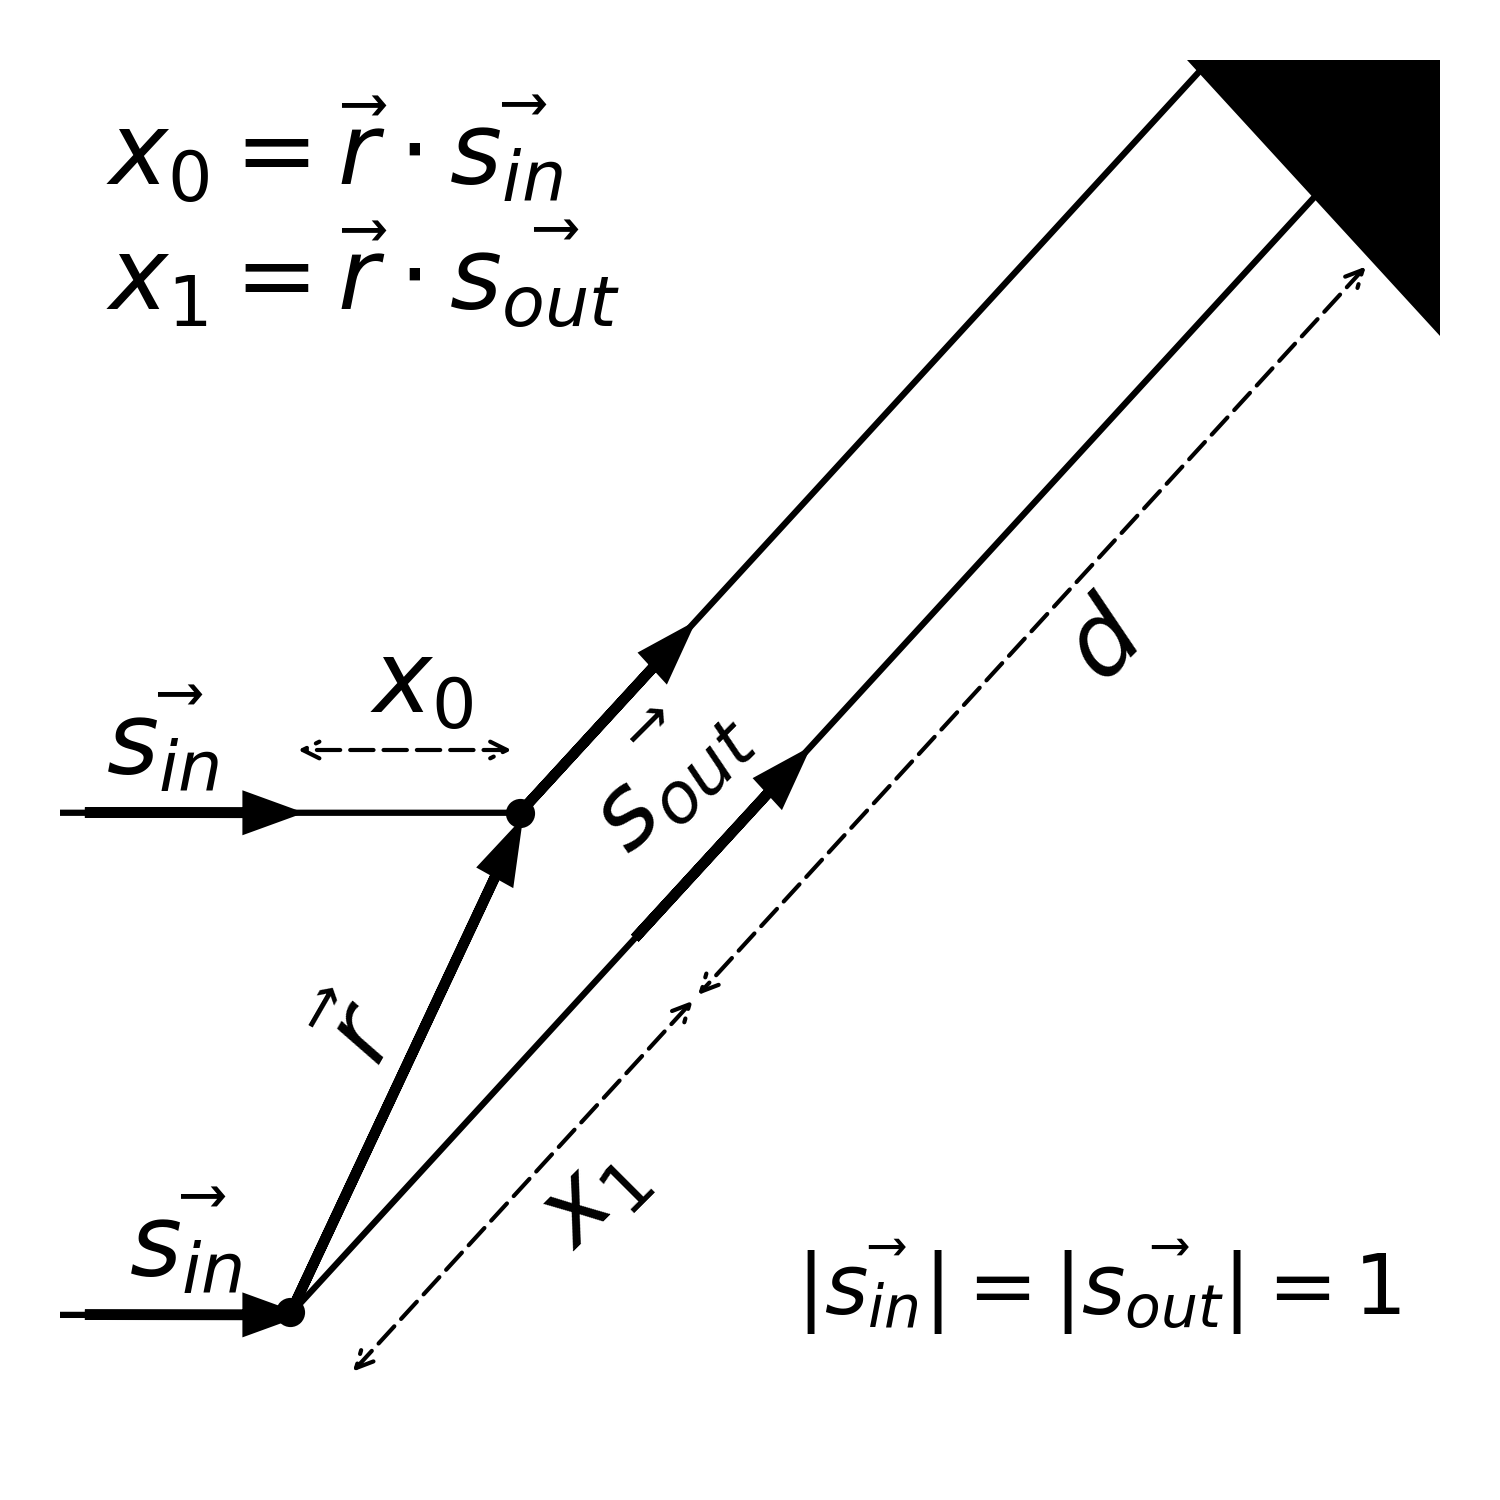
\includegraphics[width=40mm]{blah.png}
\label{fig:Interference}
\caption{Illustration of the scattering from two free-electrons. a) The two blue dots represent two independently scattering free-electrons. The rings represent the maxima of the two scattered waves. One can see the a light-dark band structure appear, characteristic of a interference pattern. b) mathematical description of the path length difference between two waves arriving at point $\vec{d}$. $\hat{s}_{in}$ and $\hat{s}_{out}$ are unit vector pointing in the direction of the incident wave and the out going wave respectively. $\vec{r}$ is a position vector describing the relative distance between the two electrons. }
\end{figure}

If the diffraction pattern is measured at point \(\vec{d}\), far away from the diffracting object itself, both scattered fields have approximately the same field strength since the distance from both electrons to the detector is about equal. In Figure \ref{fig:Interference} this means that  $|\vec{d}+x_1| \approx |\vec{d}|$, and that both $\hat{s}_out$ are parallel. This approximation is called the far-field approximation. The Fresnel number (FN) is used to verify the validity of the far-field approximation.
\begin{equation} 
FN = \frac{o^2}{d\lambda}
\end{equation}
where $o$ is the object size, $d$ the distance from the
object to the detector, and \(\lambda\) the
wavelength of the radiation. The far-field approximation is valid when $FN \ll 1$. All diffraction patterns discussed
in this thesis are taken in the far-field. 

The electric field at point $\vec{d}$ is given by a sum of the individual scattered electric fields:
\begin{equation}
E(\vec{d}) = E_s(\vec{d})+E_s(\vec{d}) e^{\frac{2 \pi\,i\,\Delta x}{\lambda}} 	 
\end{equation}
$\Delta x$ is the optical path difference between the two scattered waves due to the relative difference in position. $\Delta x$ can be determined by summing $x_0$ which is the path difference of the incoming radiation and $x_1$ which is the path difference of the outgoing radiation. Both $x_0$ and $x_1$ can be described using the difference vector $\vec{r}$: 
\begin{equation}
\Delta x = x_0 - x_1 =\hat{s}_{out} \cdot \vec{r}-\hat{ s}_{in}\cdot \vec{r} = (\hat{s}_{out} -\hat{s}_{in} ) \cdot \vec{r} 
\end{equation}

By defining the scattering vector $\vec{S}$
\begin{equation}\label{eq:ScatteringVector}
\vec{S} = \frac{\hat{s}_{out}}{\lambda} - \frac{\hat{s}_{out}}{\lambda}\\ = \vec{s_{out}}-\vec{s_{in}}
\end{equation}
the diffraction pattern of two electrons van be written as:
\begin{equation}
E(\vec{d}) = E_s(\vec{d}) + E_s(\vec{d}) e^{2\,\pi\,  i\,\vec{S}\cdot\vec{r}}
\end{equation}

Implicit in this interpretation is the assumption that the scattered field will not be scattered a second time. This approximation is called the first Born approximation. We assume this to be valid for all objects smaller than a few micrometers.

Important to note is that $\Delta x $ can be at most $|\vec{r}|$, the distance between the two electrons. Abbe demonstrated that in order to resolve two electrons from each other at least two diffraction orders must be captured. This usually means the zeroth and the first order. The first order start where $\Delta x > \lambda/2$. For two electrons closer than half a wavelength apart this will never be the case. This sets a physical limit to the possible details one can resolve using a regular diffraction set-up. One would not be able to use green light ($\lambda = 500\,nm$) to image objects smaller than 250 nm. For structural studies of molecules this means that in order to distinguish single atoms, X-ray radiation is required.

\section{Scattering from multiple electrons}
The framework for describing the scattering of two electrons can easily be extended to N electrons, considering that every electron scatters independently from the others. The electric field can be described as the sum of all the individual scattered fields.
\begin{equation}\label{eq:boehoe}
E(\vec{d}) = E_s(\vec{d}) \sum_{n} e^{2\,\pi\,  i\,\vec{S}\cdot\vec{r_n}}
\end{equation}
where n identifies the individual electrons.

In biological particles the incoming EM radiation is scattered by electrons that are part of atoms, instead of being scattered by free electrons. As we will see, this has a major effect on the scattering process. The scattering potential $\rho(\vec{r},\lambda)$ describes the scattering from a single atom in comparison to the scattering by a free electron. At X-ray wavelengths $\rho(\vec{r},\lambda)$ can be approximated by:

\begin{equation}
\rho(\lambda.\vec{r}) = -r_e (f_1 + i\,f_2)
\end{equation}
Here, $r_e$ is the classical electron radius. $f_2$ is derived from the atomic photoabsorption cross section and is a measure of absorption [booklet]. $f_2$ becomes very relevant close to an absorption edge of the material. $f_1$ describes the scattering power of an atom. It is related to the imaginary part by the Kramers-Kronig dispersion relation [Kramers]. At high photon energies $f_1$ approaches the atomic number of an atom.  

For most elements, the exact value of $f_1$ and $f_2$ have been determined experimentally for a wide range of photon-energies \cite{Henke1990}. Figure \ref{fig:waterwindow} presents the scattering factors of two elements: carbon and oxygen. The energy range from 282-533 eV (4.40 nm - 2.33 nm) is called the water window. In this region, and especially towards the higher energies, oxygen atoms and thus water, are scattering significantly less than the carbon atoms that  make up organic biomolecules. The water window is therefore a good candidate for imaging cells, as the contrast between two of their main constituents, water and biomolecules, is enhanced.

\begin{figure}[h]
\centering 
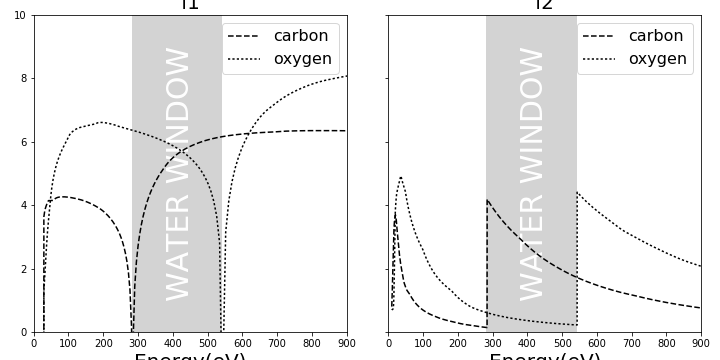
\includegraphics[width=80mm]{waterwindow.png}
\label{fig:waterwindow}
\caption{Atomic scattering factors $f_1$ and $f_2$ of carbon and oxygen, as a function of photon-energy of the X-ray radiation. The region between the absorption K-edge of carbon (282 eV, 4.40 nm) and the K-edge of oxygen (533 eV, 2.33 nm) is called the water window.  The contrast between biomolecules and water is enhanced in this region, especially towards higher photon energies. These wavelengths could be used for imaging living biological particles such as cells or organelles.}
\end{figure}

The scattered field can now be described as follows:

\begin{equation}\label{eq:boehoe2}
E(\vec{d}) = E_s(\vec{d}) \sum_{m} \rho(\lambda,\vec{r}) e^{2\,\pi\,  i\,\vec{S}\cdot\vec{r_m}}
\end{equation}
where $m$ denotes the different atoms.

If all electrons together are assumed to form a continuous electric charge density around the many nuclei that constitute the biological particle, equation \ref{eq:boehoe}  can be written as a continuous function. 

\begin{equation}\label{eq:cont}
E(\vec{d}) = E_s(\vec{d})\int \rho(\vec{r},\lambda) \exp^{-2\pi i \,\vec{S} \cdot \vec{r}}\,d\vec{r}
\end{equation}

We can now introduce the scattering factor $F(\vec{S})$.
\begin{equation}
F\left(\vec{S}\right) = \frac{E(\vec{d})}{E_s(\vec{d})} = F\left(\frac{\vec{d}}{|d|}\right)
\end{equation}
The structure factor is independent of the distance of the detector, it only depends on the angle of measurement. Instead of structure factor, the term molecular transform is often used in the field of crystallography. Throughout this thesis we will use this term as well.

Equation \ref{eq:cont} can be rewritten as:
\begin{equation}\label{eq:diff_equation}
F(\vec{S}) = \int \rho(\vec{r},\lambda) \exp^{-2\pi i \,\vec{S} \cdot \vec{r}}\,d\vec{r}
\end{equation}

This equation is very similar to a well known Fourier transformation $\mathcal{F}( g( t ) )$ []. 

\begin{equation}
 G(\omega) = \int g(t) e^{-2 \pi i \omega\, t}\,dt
\end{equation}

Equation \ref{eq:diff_equation} is very convenient as we now know that, in the far-field, the scattering of a plane wave is proportional to the Fourier transform of the scattering potential evaluated at $\vec{S}$.

We can now also define the inverse relation of \ref{eq:diff_equation}:
\begin{equation}
\rho(\vec{r}) = \mathcal{F}^{-1} ( F(\vec{S}) ) = \frac{1}{2\,\pi}\int F(S) \exp^{2\pi i \,\vec{S} \cdot \vec{r}}\,d\vec{S}
\end{equation}


\section{the Ewald Sphere}

\begin{figure}[h]
	\centering 
	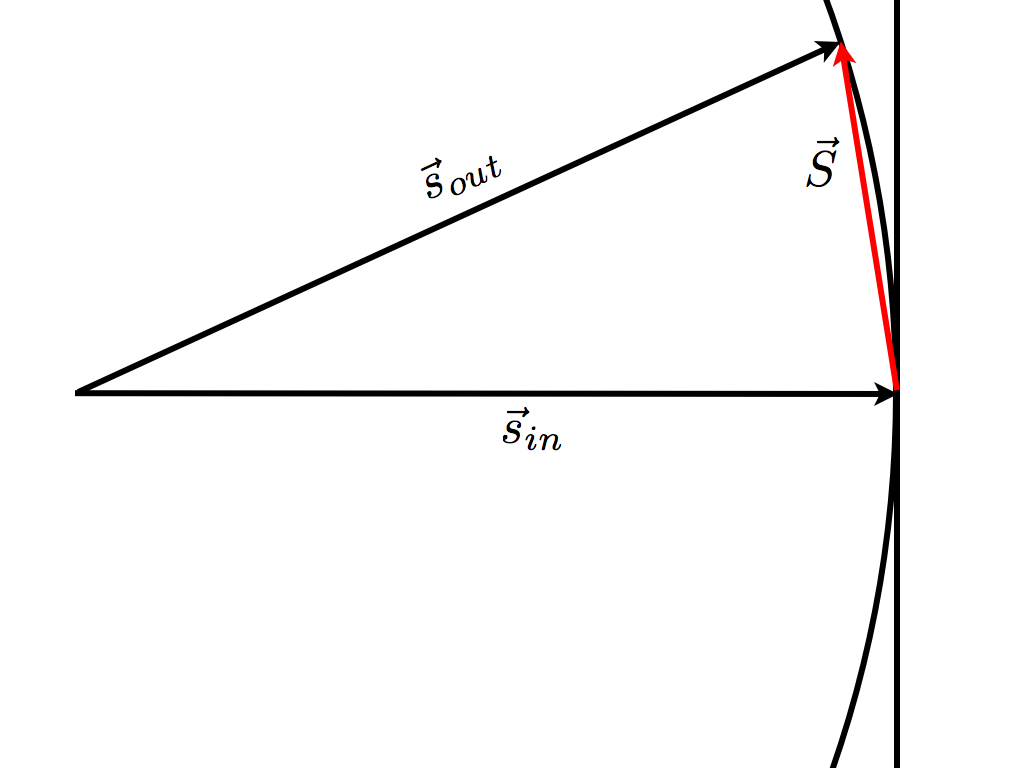
\includegraphics[width=50mm]{ewald_sphere.png}
	\label{fig:EwaldSphere}
	\caption{A schematic of the Ewald sphere. The scattering vector $\vec{S}$ will always reside on the surface of a sphere of length $1/\lambda$, that intersects with the origin of the three-dimensional molecular transform of the object. $\vec{S} = \vec{s}_{in} - \vec{s}_{out}$. $\vec{s}_{in}$ is constant and is determined by the direction of the incoming radiation. $\vec{s}_{out}$ has a constant length, but varies in direction with scattering angle $\theta$. }
\end{figure}

The molecular transform $F(\vec{S})$ of a three-dimensional object is also three-dimensional. A diffraction pattern, however, is not. To understand this, we have to evaluate $\vec{S}$ more carefully. 

In a diffraction experiment $\vec{S} = \vec{s}_{out} -\vec{s}_{in}$ (see equation \ref{eq:ScatteringVector},). $\vec{s}_{in}$ is constant, and is determined by the propagation direction of the incoming EM field. $\vec{s}_{out}$ has a fixed length ($1/\lambda$), and points in the direction of the scattered field ($\theta$). The scattering vector $\vec{S}$ is therefore limited to reside on the surface of a sphere of radius $1/\lambda$. This sphere is called the Ewald sphere [] (see Figure \ref{fig:EwaldSphere}). 


The Ewald sphere intersects the $F(S)$ through its center $F(0)$. At small scattering angles the curved Ewald sphere can considered to be flat. This means that a diffraction pattern can be approximated as slice through the center of the molecular transform.  This relation will prove itself to be very useful.

\section{Properties of the Fourier transform}
There is a large mathematical field describing the properties of Fourier transformations. A few of these relations are very useful to this thesis.
\begin{enumerate}

\item Linearity\\
	For any complex number $a$, if $h(t) = a g(t)$, then $H(\omega) = a \, G(\omega)$

\item Scaling\\
	For any non-zero real number $a$, if $h(t) = g(a t)$, then $H(\omega) = \frac{1}{|a|} G\left(\frac{\omega}{a}\right)$

\item Translation\\
	For any real number $t_0$, if $h(t) = a g(t+\Delta t)$, then $H(\omega) = e^{2\pi\,i\,\Delta t \omega} G(\omega)$. The factor $e^{2 \pi i \Delta t \omega}$ is called a 'phase-ramp'.

\item Convolution\\
The Convolution theorem states that a multiplication in Fourier space is a convolution in object space (real space) and vice versa.
\begin{equation}
f(t) * g(t) = \int f(\tau)g(t-\tau)\,d\tau = \mathcal{F}^{-1} \left( \mathcal{F}(f(t))\,\mathcal{F}(g(t))\right)
\end{equation}

\item {Projection Approximation}\\
The projection slice theorem states that the Fourier transform of the projection of an three-dimensional function g(t) onto an two-dimensional plane is equal to an two-dimensional slice through the origin of the three-dimensional Fourier transform of the function g(t)
which is parallel to the projection plane. At small scattering angles, a diffraction pattern is a slice through the center of the three-dimensional Fourier transform. In this case the results of equation can be interpreted as a projection of the scattering potential. 

\item {Discrete Fourier Transform}\\
In practice we are dealing with a signals that are not continuous, but discrete. Most signal recording is done digitally, and to be able to do numerical computations on the signal, it has to be digitized as well. For discrete signal the discrete Fourier transform (DFT) and the inverse discrete Fourier transform (IDFT) can be used.

\begin{equation}
DFT( g( T_{k,l,m} ) ) = G( \Omega_{k,l,m} ) = \sum_{k=1}^{K} \sum_{l=1}^{L} \sum_{m=1}^{M} g( T_{k,l,m} ) e^{-2 \pi i \Omega_{k,l,m} \cdot T_{k,l,m}}
\end{equation}

\begin{equation}
IDFT( G( \Omega_{k,l,m} ) ) = g ( T_{i,j,k} ) = \frac{1}{{K L M}} \sum_{k=1}^{K} \sum_{l=1}^{L}\sum_{m=1}^{M} G( \Omega_{k,l,m} ) e^{2 \pi i \Omega_{k,l,m} \cdot T_{k,l,m} }
\end{equation}

where $K$,$L$ and $M$ are the number of 3D pixels (voxels) in each dimensions. $T_{k,l,m}$ and $\Omega_{k,l,m}$ are the discretized version of $t$ and $\omega$. 

\end{enumerate}

\section{Radiation Damage}
The scattering power of an object is proportional to its volume, and thus varies with the 3rd power of its size. The smaller an object is, the less scattering occurs. To compensate for this loss in scattered signal, the required dose for imaging increases. Practically this means that a dose in excess of 100 MGy is required to record an interpretable signal from a living cell. To put this in perspective, a dose of 2000 Gy is already enough to kill an organism that lives on earth. This means that the amount of energy deposited into the system through photoabsorption is not negligible. The main process of photoabsorption at soft-X-ray wavelengths is  photoionisation. Many process follow the ionization event, of which non-radiative Auger decay can lead to significant radiation damage throughout the material. The relation between the required dose of radiation versus the maximum tolerable dose of radiation posed a physical limit to the obtained resolution for imaging single biomolecules [Howell].

\section{Diffract-before-destroy}
An elegant solution to the problem of radiation damage came from the realization that elastic scattering occurs on a  time scale shorter than the damage processes manifest themselves structurally. This principle is of diffract-before-destroy, suggested in 2000 by Neutze \textit{et al.} \cite{Neutze2000}, was experimentally demonstrated on a silicon-nitrate sample \cite{Chapman2009}. This experiment used the ultra short and extremely bright pulses from the first x-ray free-electron laser to outrun key damage processes \cite{Chapman2000}. Although the pulse literally obliterated the sample, enough structural information was captured to retrieve the original structure. A single XFEL pulse has a power densities of $10^{16} W/cm^2$, and can be between 1-100 fs long. This facilitates the imaging of single particles at room temperature.

Diffract-before-destroy has been further validated by a wide variety of experiments \cite{Seibert2009,Seibert2010}. Serial femtosecond crystallography (SFX) showed that with this principle at least three orders of magnitude higher radiation doses are tolerated compared to regular crystallography, enabling the imaging of much smaller crystals []. The imaging of single particle has been shown feasible in 2D for a wide variety of biological particles, ranging from \textit{living} cells (\textbf{Paper I}) to cell organelles (\textbf{Paper VXIII}) to  40 nm viruses (\textbf{Paper XIV}). \textbf{Paper XVII} shows the experimental feasibility of using many 2D images to construct a 3D model of a giant virus.

The field is very close to measuring the first 2D diffraction patterns of single proteins. For simulated data it has been shown that such patterns can be used to recover the 3D shape of proteins, even though the number of scattered photons might be as low a 1000 photons per frame. The ultra short pulses also allow for the studying of the dynamics of such systems, either by separating the images from different naturally occurring conformational states, or by identifying structural changes subsequent to an external trigger []. In the more distant future these structural changes might be tracked inside living cells. 
 
    \chapter{Pulse Generation by XFEL}
Free-electron lasers (XFELs), invented by J. Madey and demonstrated experimentally in the 1970s, can generate multi gigawatt and femtosecond (fs) x-ray radiation. Compared to fourth generation synchrotrons, this is a ten billion-time increase in brightness. Typically an XFEL consists of three sections: i) the electron gun, ii) a linear accelerator, and iii) an undulator. The x-ray radiation is generated in the undulator. Figure 1 shows a schematic of the XFEL at the Linear Accelerator Coherent Light Source (LCLS) at Stanford. This chapter will describe the operating of the LCLS in specific. Other XFELs might use different hardware, but the fundamental principles that drive an XFEL will be very similar. Please note that the words bunch and pulse are used to discriminate between a collection of electrons and radiation respectively.

\begin{figure}[h]\label{fig:LCLS}
\centering
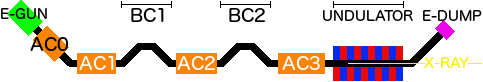
\includegraphics[width=100mm]{LCLS_schematic.png}
\caption{Schematic of LCLS. Electron bunches are created by the electron gun (E-gun). The bunches are consecutively accellerated by linear accelerators (AC0-3) and compressed by bunchcompressors (BC0-1). After the final acceleration the bunch is guided into the undulator, where an x-ray pulse is generated. After the undulator the x-ray pulse continuous to the beamline, and the electron bunch is dumped (E-dump).}
\end{figure}

In the electron gun, a copper plate is irradiated by a powerful ultraviolet laser pulse, which releases a bunch of electrons. At this moment the electron bunch is a few picoseconds long and has a peak current less than 100 A. As shown in figure \ref{fig:AC}a, the energy spread within the bunch is minimal at this point. The electron bunch is directly accelerated to 99.7\% of the speed of light, using a standing wave in a RF cavity (AC0). Due to cooling reasons in AC0 the LCLS produces electron pulses at maximally 120 Hz. 

\section{Klystron}

Consecutively the bunches are guided in a long series of accellerating units named klystrons. See AC1-3 in figure \ref{fig:LCLS}, and for more detail figure\ref{fig:AC})d. In essence a klystron is a cylinder on which an strong MHz alternating current is applied. The AC current induces a EM field in the MHz range (RF), similar to the way radiowaves are produced in an antenna. Due to the spacing between irises the relative phase velocity of the wave is matched to the speed of the electrons, thus through the Lorentz force longitunal acceleration can be achieved throughout the whole klystron. In the center of the cavity the magnetic field is zero, the acceleration is therefore proportional to the strength of the electric field. Each klystron can maximally add 30 MW/m of energy to the electron bunch. Under higher currents the klystron will tear itself apart. In order to reach 15 GeV electron bunches at least 500 m of klystrons are needed. In reality the accelerating unit of LCLS are 889 m long. Often accelerators do not operate at the point of maximum acceleration, since one wants to introduce a negative energy gradient along the particle bunch, that can later be utilized for bunch compression. This acceleration method is called off-crest acceleration, and is visualized in figure  \ref{fig:AC} b and d. A negative energy gradient means that the electrons located at the front of the bunch have a slightly lower energy compered to electrons the electrons are located at the rear of the bunch.

\begin{figure}[h]\label{fig:AC}
\centering
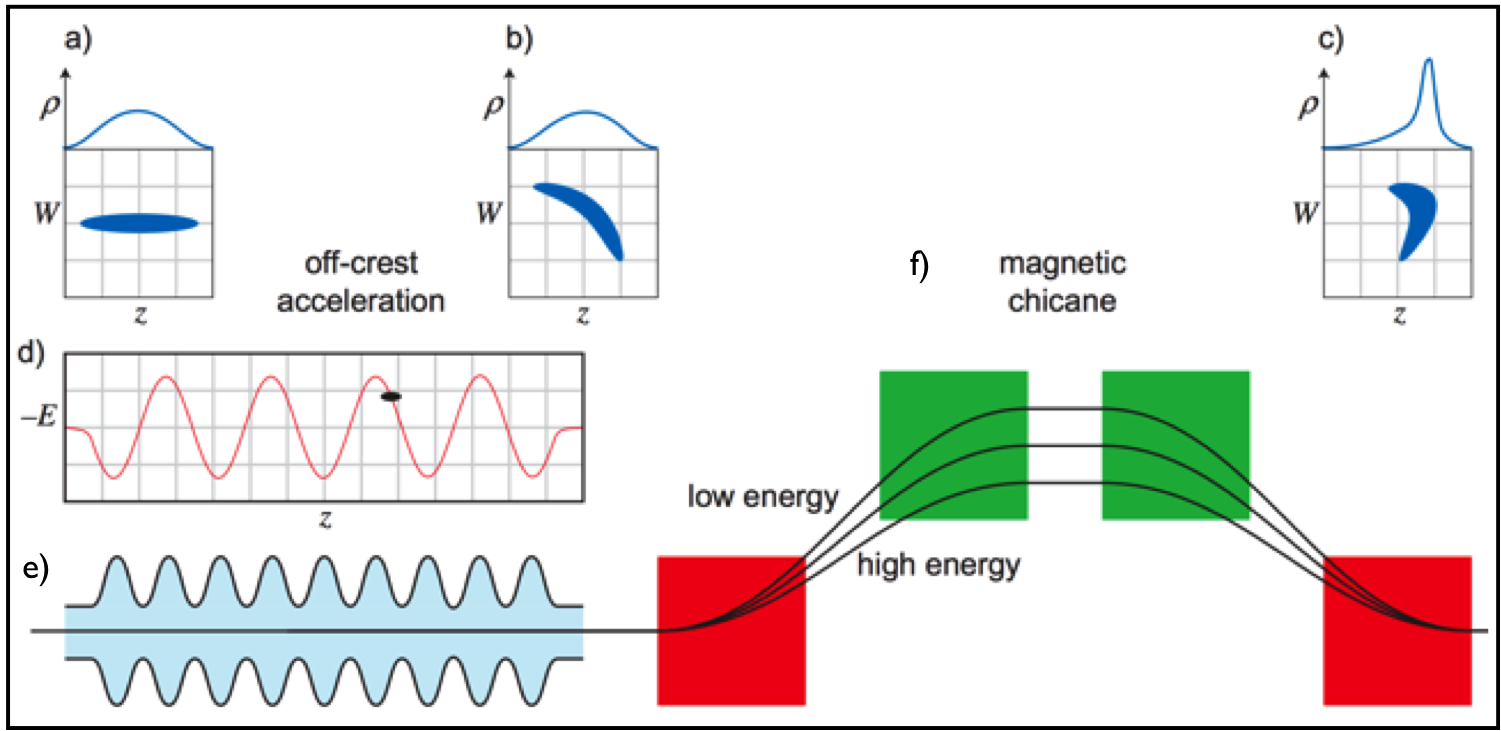
\includegraphics[width=100mm]{acceleration.png}
\caption{Schematic of Acceleration and bunch compression at LCLS. a-c) change of bunch shape throughout the accelerator. d) illustration of the off-crest accelleration principle. a) shows that  This creates an energy chirp. e) schematic of a single klystron. f) schematic of a chicane. The green and red blocks are magnetic dipoles that deflect the electron bunch in opposite direction. The path of high energy electrons diverges less than lower energy electrons. If the bunch has a negative energy chirp, this results in bunch compression.}
\end{figure}

\section{Bunch Compression}
Short and compact bunches are essential for the functioning of an XFEL. One of the main bunch-compression devices are chicanes. Chicanes consist of four magnetic dipoles that diverge the high energy part of the bunch less than the low energy part (see figure \ref{fig:AC} ). Due to the negative energy gradient it thus reduces the temporal spread of the bunch. After the final compression the electron bunch is ~40fs long, has a peak current of 4.3 kA, and travels at 99.999\% of the speed of light. The relastivistic $\gamma \sim 2000$. Creating these type of bunches is a noteworthy technical achievement, 

\section{Undulator}
\subsection{Monochromatic X-ray radiation}
The undulator is the heart of an XFEL. It is a periodic arrangement of magnets with alternating poles. The magnetic field of a periodic magnetic structure can be written as:
\begin{equation}\vec{B}(z) = B_0\cos{(\frac{2\pi}{\lambda_u}z)}\hat{\mathbf{y}}\label{eq:bz}\end{equation}
$B_0$ is the magnetic field, $\lambda_u$ is the wavelength of an undulator period.
Due to the magnetic field the moving bunch of electrons experience a Lorentz force, causing it to oscillate in the transverse direction (x). The movement can be described by the following equation. 
%\begin{equation}\vec{F} = e(\vec{v}\times\vec{B})\end{equation}
\begin{equation}v_x = \frac{-e\,B_0\,\lambda_u}{2\pi\,m_e\gamma} \sin{(\frac{2\pi}{\lambda_u}z)} = \frac{K c}{\gamma} \sin{(k_uz)}\label{eq:vx}\end{equation}
Usually the non-dimensional parameter K is written as:
\[K =  \frac{-e\,B_0\,\lambda_u}{2\pi\,m_e \, c}  \approx 0.9337 B_0 \lambda_u\]
where the magnetic field is measured in Tesla and the undulator period in centimeters.

Preserving momentum the oscillating electrons emit radiation ($\lambda_s$). As described in chapter 1, interference effects will occur between the emitted waves from the different charges (remember the electrons come in a bunch which has a size). The essence of this interference phenomenon lies in the longer route taken  by the oscillating electrons compared to the radiation, which causes an OPD between the radiation emitted by electrons one undulator period apart. If the OPD between the electrons and the radiation is equal to and integer of $\lambda_s$, the emitted waves will add coherently. Radiation with other wavelengths will interfere destructively. The longer an undulator the more pronounced the selection of specific wavelengths. Equation \ref{eq:res} describes this so-called resonance condition.%, as shown in figure 3b.
\begin{equation}c\frac{\lambda_u}{<v_z>} -\lambda_u\, \cos{(\theta)} = n \lambda_s \label{eq:res}\end{equation}
To predict at which wavelength this happens we need to find the average longitudinal velocity $v_z$. As the total speed $v$ of the electrons is not affected by the Lorentz force, $v_z = \sqrt{ {v}^2-{v_x}^2}$\footnote{Using Pythagoras' theorem}. Using Equation \ref{eq:vx} for $v_x$ and $\gamma^2 \equiv (1-\frac{v^2}{c^2})^{-1}$, we can write $v_z$ as: 
\[ v_z = \sqrt{c^2(1-\frac{1}{\gamma^2})-\frac{K^2 c^2}{\gamma^2}\sin^2(k_u\,z)} = c \sqrt{1-\frac{1}{\gamma^2}(1-K^2\sin^2(k_u\,z))}\]
Using the mathematical identity $\frac{1}{\pi}\int_{0}^{\pi} \sin^2( x ) \, dx =\frac{1}{2} $, integrating of half a undulater period gives the average velocity $<v_z>$.
\[<v_z> = c\sqrt{1-\frac{1}{\gamma^2}(1-\frac{K^2}{2})}\]
${\gamma} \gg 1$, thus we can expand the root $\sqrt{1+x} = 1+\frac{1}{2}x-\frac{1}{8}x^2+ ...$ (first order Taylor expansion).
\[<v_z> \approx c(1-\frac{1}{2\gamma^2}(1+\frac{K^2}{2}) )\]
If we now assume that we only observe the radiation in the forward direction, we can expand $\cos{(\theta)} = 1-\frac{\theta^2}{2}$. 
Equation \ref{eq:res} can thus be written as:
\[ n \lambda_s = \lambda_u[\frac{1}{1-\frac{1}{2 \gamma^2}(1+\frac{K^2}{2})} - (1-\frac{\theta^2}{2})]\]
The geometrical series $\frac{1}{1-x} = 1+x+x^2+...$ allows us to obtain the well known undulator equation.
\begin{equation} n \lambda_s = \frac{\lambda_u}{2 \gamma^2}(1+\frac{K^2}{2}+(\gamma\theta)^2)\end{equation} 

This formula can be explained by two relativistic effects. For an observer it is the electron bunch that is moving close to the speed of light. In the electron bunch's frame of reference however it is the undulator that is moving very fast. Fast objects are length contracted, thus the electrons observes a undulator period of $\frac{\lambda_u}{\gamma}$, which makes it emit radiation with $\lambda$ around $\frac{c\lambda_u}{\gamma}$. The radiation is relativistically contracted when observed in the laboratory's frame of reference (relativistic doppler effect), adding the second gamma term. The size of relativistic doppler effect is dependent on the angle of observation relative to the direction of motion. 

The final wavelength of the emitted light is thus dependent on the energy of the electrons ($v$), the magnetic field in the undulator ($B$), and the angle of observation ($\theta$). Control over these variables makes the selection of a specific wavelength possible. LCLS can produce X-ray radiation in the range of 400 eV -10 keV. 


%\subsection{Direction of Emission}
\subsection{SASE}
So far the emitted radiation is monochromatic, but not temporally coherent. This means the total emitted power is proportional to the number of the electrons in the bunch ($N_e$). If all emitted radiation would emit in phase, the total irradiated power would be proportional to ${N_e}^2$. Pellegrini and others realized that for short pulses, and long undulators, temporal coherence could by achieved by a process called Self Amplified Stimulated Emission (SASE). SASE exploit the slight non-uniformities in the electron bunch, that cause radiation with a certain phase to be slightly more prevalent than others. The Coulombic force exerted by the electric field of this radiation will start grouping electrons at its nodes (See figure 2). Electrons are accelerated when the electric field is positive, and decelerated when negative, causing the so-called microbunches to appear. This process forms a positive feedback loop, causing a exponential increase in radiation power. The  exponential  growth  cannot  continue  indefinitely, and  the  power  must  saturate  at  a  certain  level. The SASE process ultimately saturates when either the electrons loose so much energy the resonance condition is not met anymore, or when the energy of the radiation surpasses that of the electron bunch. In the latter case the EM wave will start to transfer energy to the electron bunch instead\footnote{This phenomenon is similar to inverse Compton scattering, in which electrons absorb energy from the radiation field.}.

The high power density within the pulse means that there are more than one photon in the volume of a $\lambda^3$. Which means that so far diffraction patterns come from single photons interfering with themselves []. Interference between more than one photon might be different. For example there might be special interactions between photons. 

\section{Improvements}

Seeding
Multi-angle
High rep rate





    \chapter{Sample Introduction}
This chapter will discuss different methods of delivering sample into the x-ray pulse. Sample delivery can be divided into roughly two classes: substrate-bound and substrate free sample delivery. Figure \ref{fig:experimental_geometry} shows a schematic of a general set-up of an experiment, including several sample delivery systems. Usually one sample delivery system is chosen, which is aligned such that the sample and the beam intersect. If the x-ray pulse intersect with the sample (and/or substrate) a diffraction pattern is recorded on one or two sets of detectors, placed at different distances from the interaction region.

It is important to note that the whole system is under reduced pressure, $10^{-6}$ mbar. This is done to reduce the background scattering from the gas molecules themselves. Pumping a chamber down to $10^{-6}$ mbar takes hours, and is a factor which has to be taken into account in the planning of the experiment. 

\begin{figure}[h]\label{fig:experimental_geometry}
\centering 
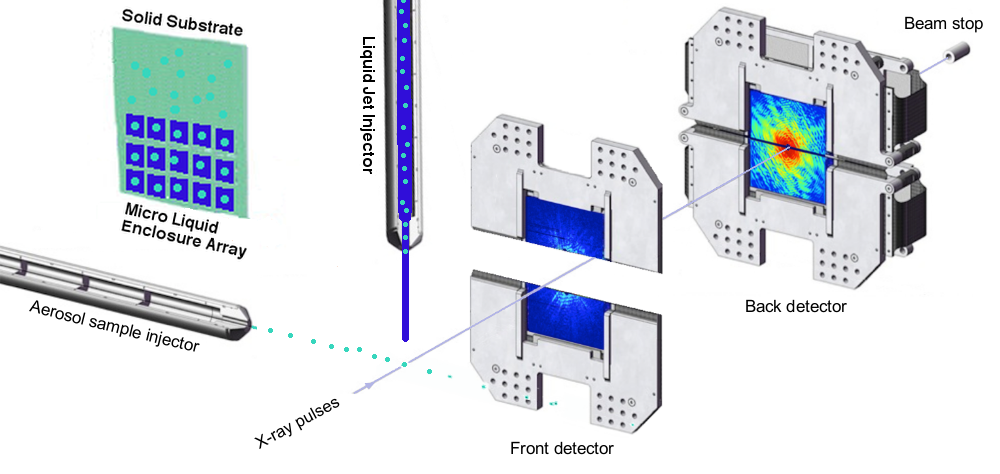
\includegraphics[width=90mm]{setup_cropped.png}
\caption{Experimental geometry, including different sample delivery system. From the bottom left the x-rays pulses enter the chamber. The experimentalist can now select a sample delivery system. Shown are an aerosol sample delivery system, liquid jet injection system, and two types of substrate bound sample delivery systems. If the beam intersect the sample (and/or substrate) a diffraction pattern is recorded on two sets of detectors, placed at different distances from the interaction region.}
\end{figure}

\section{Substrate-bound Sample Delivery}
\subsection{Solid substrate}
One of the easiest ways of introducing samples is by attaching them to a solid surface. Shortly after the operation of the first XFEL (FLASH) the principle of diffract-before-destroy was demonstrated on a inorganic sample attached to a fixed membrane [Chapman]. Soon after the first cells were imaged on a silicon-nitrate window. The main disadvantages of this sample delivery system are i)the sample has to be able to tolerate prolonged exposure to reduced pressure, ii) the substrate causes significant background scattering, and iii) the repetition rate is limited by the time it takes to mechanically move the solid substrate from one position to the next. The latter becomes a significant problem at the high repetition rate XFEL sources.

\subsection{Micro Compartments}
In order to circumvent the problem of the prolonged exposure to the vacuum, a system called Micro Liquid Enclosure Array (MLEA) can be used. A MLEA system consists of an array of micro-compartments filled with liquid attached to a regular grid (see figure \ref{fig:experimental_geometry}. The microcompartments are closed off with by a membrane. This method has been successfully used in the imaging of cells. Getting your sample into the microcompartments is tedious and time consuming. The liquid in the microcompartments produces significant background scattering. 

\subsection{Liquid Jets}

Liquid jet systems can produce stable streams of particles in solution. Mainly two types of liquid jet nozzles are used for sample injection into the XFEL pulse train: i) liquid nozzles (Rayleigh jets), ii) liquid nozzles assisted by coaxial gas flow also referred to as gas dynamic virtual nozzle (GDVN). 

Vacuum compatible systems of the Rayleigh jets with diameters ranging approximately from 5 to 100 $\mu m$
exist. Typical liquid flow velocities of such jets is 120 m/s. The sample consumption within such a jet is in the order of ml/s. For many biological samples this rate of sample consumption is too high. Sample consumption can be reduced by slowing down the stream or by reducing the diameter of the nozzle. However, for orifice diameters smaller than 10 $\mu m$, clogging of the nozzles becomes a serious issue. To reduce the jet diameter without the danger of clogging the sample delivery, GDVN liquid jets were introduced [DePonte]. In a GDVN nozzle a coaxial stream of high velocity He gas is used to accelerate the liquid stream. Similar to the flow of water from a tab, the accelerating stream is reduced in diameter. Jet diameters below 1 $\mu m$ have been recently achieved [W]. 

Liquid jets have the advantage to study biological samples in their natural environment, to refresh the sample throughout the experiment with sample consumption in the order of 10 $\mu l$/min [Weierstall 2012], and allows for imaging at high repetition rates. This GDVN setup is commonly used in serial femtosecond crystallography (SFX) experiments. The Bragg peaks of nano crystals are sufficiently strong to surmount the background scattering from the surrounding jet.

\section{Substrate-free sample delivery}
In FXI everything that is illuminated by the X-ray pulse is sample, including the structure of the sample holder, the liquid column of a liquid jet, or materials that make up microfluidic devices. Such sample holders contribute to scattering and increase unwanted noise. Especially for weakly scattering single particles the noise might drown the signal. Aerosol injection removes this clutter and assures that the sample is clearly isolated from its surroundings, and this is, as we see in a later chapter, important for image recovery.

An aerosol injector produces small droplets of particles dissolved in a volatile buffer, typically ammonium acetate. The buffer evaporates under the reduced pressure, ideally leaving behind only the particle. There are two main types of nozzles that can be used to produce small drops: the Gas Dynamic Virtual Nozzle, and electro spray ionisation (ESI).

\subsection{Gas Dynamic Virtual Nozzle}

If the coaxial flow of gas creates a jet with a diameter smaller than then a characteristic $d_j$ the surface tension in the liquid will cause the jet to break up into a mist of small droplets. $d_j$ can be estimated on the basis of energy conservation, and is a function of the effective pressure drop $\Delta P$. It is assumed that all energy is transformed to kinetic energy [Calvo].
\begin{equation}
d_j^{(GDVN)} = 2 \sqrt{Q \cdot \left(\frac{\rho}{2 \pi^2 \Delta P}\right)^{1/2}}
\end{equation}    
$Q$ denotes the flow rate and $\rho$ is the density of the liquid. The final drop diameter $d_d$ can be related to the jet diameter using the ratio $d_d / d_j \approx 1.9$, which is the classical Rayleigh breakup []. Empirically this assumption has shown to work well for low viscosity media such as water. The GDVN can create droplets in the size range of 400 nm - 2000 nm. Sample consumption is in the range of ul/min.

\subsection{Aerodynamic Lens Stack}
After the droplets formed, they start to evaporate in the reduced pressure environment, leaving only the non-volatile particles in the 'drop'. The aerosolised particles are guided into an aerodynamic lens stack (see figure ). This is a series of cylindrical cavities, connected by co-aligned orifices, that collimate the droplets into a narrow beam of particles [].

For robust particles, which are large compared to the drop size, this type of sample injection has shown to be very successful. This sample injection method really opened up the possibility to measure the diffraction pattern of isolated single particles at high signal-to-noise ratios at very high repetition rates. Up to 80\% hit ratios of the 120 Hz repetition rates of the LCLS have been recorded [Hantke]. The results discussed in this thesis come from datasets that were generated using the GVDN injection method.

For many samples aerosol injection is not disruptive. Molecular dynamics simulation have shown that the conformation of proteins is conserved up till the moment that the last structural water evaporates[]. For the cyanobacterial cells described in this paper it has been shown that the shape and the autofluorescence properties of the cell membranes of the injected cells remain unchanged [PAPER I]. This is not quite unexpected. Aerosols of cyanobacteria can be carried for long distances, and metabolically active cells have been detected at altitudes of 20-70 km where atmospheric pressure drops to below a millibar []. Other sample cell lines such as E coli and brewers yeast, or many types of viruses have shown to be viable after injection. Nevertheless, not all sample types may be amenable to aerosol sample injection, and any sample type should be tested prior to experiments.  

\subsection{Electro Spray Ionisation}
Over the last years it became apparent that GDVN sample injection does have its limitations. If the particle becomes small compared to the drop size, wide size distributions of otherwise uniformly sized particles were measured [Daurer, Hantke]. These observations might be explained by a combination of an incomplete evaporation process, and the build up a significant shell of debris, originating from impurities present in the solution, around the particle. To purify the measured sample, smaller drops had to be generated. A common aerosolisation technique used in mass spectrometry called electro spray ionisation (ESI) is known to be able to produce small droplets.

ESI nozzles produce droplets through a similar droplet formation process as occurs in the GDVN. The difference lies in the process that drives jet acceleration. In ESI the jet is accelerated by an externally applied electrostatic potential. In the capillary the solvent (volatile buffer) is mixed with negatively charged ions. By applying an external field these ions are accelerated, accelerating the entire jet. The accelerated jet will ultimately break into small drops similar as happens in a GDVN. The characteristic $d_j^{ESI}$ can be described as a function of the surface tension $\sigma$, vacuum permittivity $\varepsilon_0$, electrical conductivity $C$, as well as the flow rate and the density of the liquid.
\begin{equation}
d_j^{(ESI)} \approx 2 \sqrt{Q \cdot \left(\frac{\rho \varepsilon_0}{\sigma C}\right)^{1/3}}
\end{equation}

After the process of evaporation initiates an electric potential starts to further build up in the drops, eventually leading to a coulomb explosions of the drops [Cole]. Cycles of evarporation and explosion leads to smaller and smaller drops. Initial experiments showed that drops of mono disperse droplets of size 150-200 nm can be generated with ESI. ESI can be combined with an aerodynamic lens stack as well. 

The transfer of ESI to FXI is a considerable achievement that will allow the field to move forward to image smaller particles such as proteins. This would not have been possible using the GDVN aerosolisation. ESI has been shown to also function under lower flowrates, allowing to reduce sample consumption to 10 nl/min []. This sample consumption rate is compatible with samples that are only available in small quantities. 

\subsection{Drop-on-demand}
The combination of ESI and a quadrupole with an ion trap for storage allows for a pulsed delivery system that can be tuned to match the repetition rate of the XFEL. This is generally referred to as drop-on-demand. This would reduce the sample consumption even further. Moreover the ion trap can also be utilized for sample selection prior to injection of sample into the x-ray pulse. This is important for single proteins as they scatter very little signal, which makes it very difficult to separate diffraction patterns from the real particle from diffraction patterns from potential contamination. 


    \chapter{Data recording}
As we have learned in chapter 2, a diffraction pattern is the Fourier transform of the scattering potential, sampled at the Ewald sphere ($F{\vec{S}}$). The scattering potential is determined by the structure of the object which is sampled. If a diffraction pattern measures the low scattering angles, the curved Ewald sphere might be approximated as being flat. This chapter will describe the essentials of the process of actually measuring the diffracted signal.

The value of $F{\vec{S}}$ is complex. The complex amplitude corresponds to the amplitude of the measured wave, and the complex argument corresponds to the phase shift of the wave.
Currently no device exists capable of measuring the phase of x-rays directly, as it changes in the attosecond range. The amplitude of the EM wave can be determined through an intensity measurement. 

\begin{equation}
I(\vec{S}) = |F(\vec{S})|^2
\end{equation}

In the experiments described in this thesis we used a so-called pnCCD detector to determine the $I(\vec{S})$. A pnCCD is a 2D array of pixels of size $p$. Each pixel registers the intensity of the EM wave at that location by converting the energy present in the EM wave into an electrical current, using a physical process called the photo-electric effect (a type of photoabsorption). 

$F(\vec{S})$ is independent from detector distance $d$, while a diffraction pattern is not. The relative scaling factor between the two is $\frac{1}{\lambda\,d}$. This means that the area covered by a pixel of size $p$ on the detector covers an area of size $q = \frac{p}{\lambda \, d}$ of the Ewald sphere (given the small angle approximation holds). 


Using the scaling relation between $F(\vec{S})$ sampled at the Ewald sphere, and the measured diffraction pattern at the detector, we can derive that pixel $P$ on the detector corresponds to pixel $\vec{Q} = \frac{\vec{P}}{\lambda\,d}$ on the Ewald sphere. 

Since $F(\vec{S})$ is measured at discrete locations, we have to use the discrete Fourier transform (DFT), and its inverse, to describe the relation between the measured diffraction pattern and the scattering potential. From now on we will use $F(\vec{Q})$ to describe $F(\vec{S})$ measured at discrete positions. 

The use of the DFT implies that the scattering potential is also discretized. The pixel size in real space (scattering potential space) $r$ is the inverse of the size of the detector in Fourier space ($D$). $D = n\,q$, where $n$ in the number of pixels on the detector, $q$ is the size of a pixel on the Ewald sphere. $q$ is the scaled version of a detectro pixel $q = \frac{p}{\lambda d}$. This makes $r$
\begin{equation}
r = \frac{\lambda\,d}{n\,p}
\end{equation}
Here $\lambda$ is the wavelength of the radiation, $d$ the detector distance, and $p$ is the size of a detector pixel.

%In a measurement the energy of a EM wave appears quantized, which means that one will always measure an integer number of the basic quantum of radiation: photons. The energy of a photon is related to its wavelength. The quantisation the measured intensity also has as an effect on the statistics, as they ar

\section{Missing Data}
The geometry of the detectors used in the experiments described in this thesis consist of two moveable halves (38.4 mm by 76.8 mm), with a dead area of at least 0.8 mm in between both halves (see figure \ref{fig:experimental_geometry}). In the center of the
detector a hole is created to let the high-intensity direct beam through (each detector halve misses a semicircle). For both the dead area, and the central hole no intensity information present. As a result the diffraction pattern is incomplete. 

In some experiments two pairs of detectors are used, in which one pair located closer to the sample (see figure \ref{fig:experimental_geometry}). The back detector is closed, and the front detector is opened such that is does not shadow the back detector.
 
\section{Saturation}
Besides missing data due to the detector geometry, detector saturation might also lead to missing information. Each pixel on the detector can maximally hold a certain amount of electrical charge. If more charge is present in the pixel, the excess charge will overflows to neighbouring pixels, making it impossible to accurately use the original and the
affected pixels. If the amount of charge is very high, saturation might even damage the detector itself. Saturation usually occurs in the center of the detector, because these regions are typically the most intense regions of a diffraction pattern. 





    \chapter{Phase Retrieval}
The problem of missing phase information is well known and is called the phase problem. There are many ways to overcome it: for example in crystallography homology modelling or the anomalous scattering of heavy atoms is exploited to retrieve phases. Holography uses the interference between two wave fields to obtain the phases. Ptychography uses the precisely known overlap and high redundancy between many exposures to solve the phase problem. CXI makes use of the fact that pnCCD detectors so-called oversample the diffraction pattern, which means that phases can under certain conditions be retrieved from the intensity pattern itself. The next sections will describe oversampling in more detail, explain how phases can be retrieved from an oversampled signal using an iterative phase retrieval method, and finally how phase retrieval can be validated. 

\section{Oversampling} 
In 1952 Sayre noticed that the Bragg peaks sample the molecular transform $\mathcal{F}(H)$ at the critical sampling rate ($S_C$)\cite{Sayre1952a} (See Shannon \cite{Shannon1949a}). This means that knowing the phases belonging to the Bragg peaks is just enough to back-calculate the structure of the measured object. Single particle imaging is free from the crystal lattice, and isolated Bragg peaks give way to a continuous diffraction pattern. By choosing the detector distance appropriately such that individual pixels cover a small enough angle, we can sample the molecular transform more finely than the critical sampling rate. This sampling condition is called oversampling. Figure \ref{fig:sampling} illustrates both cases of sampling. 

\begin{figure}[h]
	\centering 
		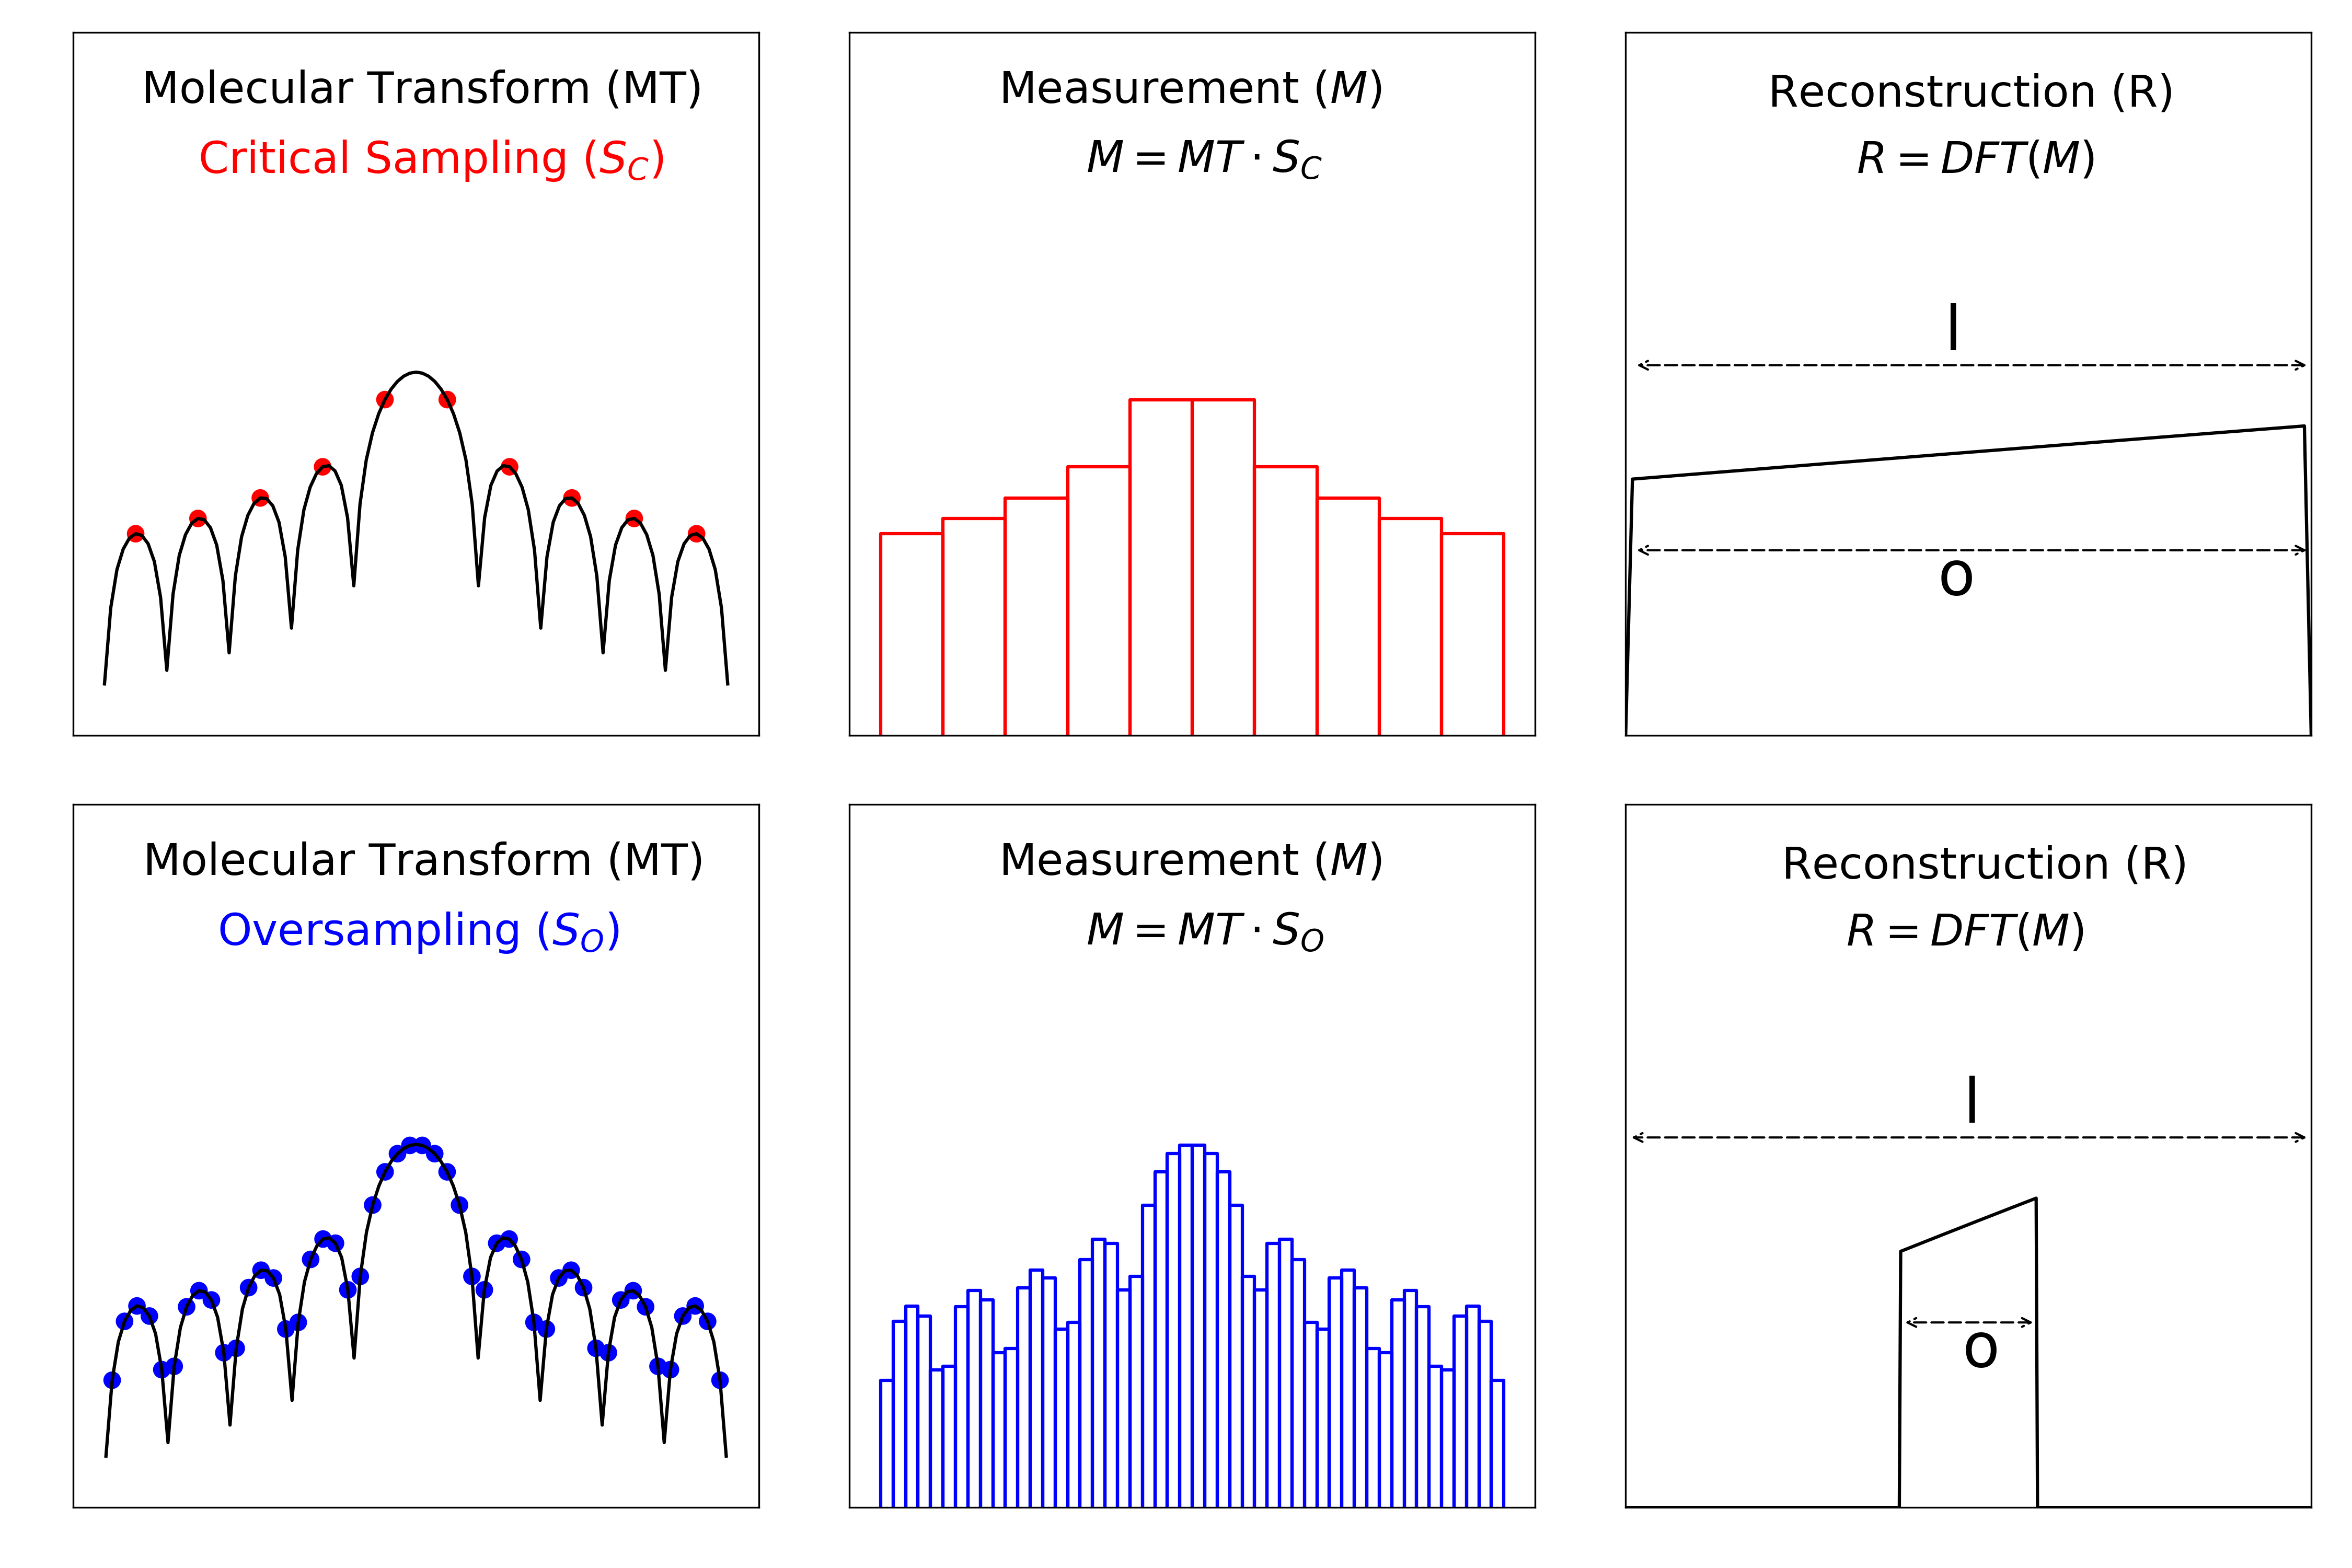
\includegraphics[width=120mm]{sampling.png}
	\caption{Illustration of critical sampling versus 		oversampling.}
	\label{fig:sampling}
\end{figure}

The linear sampling rate $S$ is defined as the ratio of $l/o$, where $l$ is the window size, and $o$ is the object size. Due to the inverse relation between the object and the molecular transform $l = \frac{1}{q} = \frac{\lambda\, d}{p}$, where $q$ is a 'pixel' in F(S) (see equation \ref{eq:q}. 
\begin{equation}
S = \frac{\lambda\,d}{o\,p}
\end{equation}

Figure \ref{fig:sampling} illustrates two types of sampling: critical sampling, and oversampling.

\begin{figure}[h]
	\centering 
		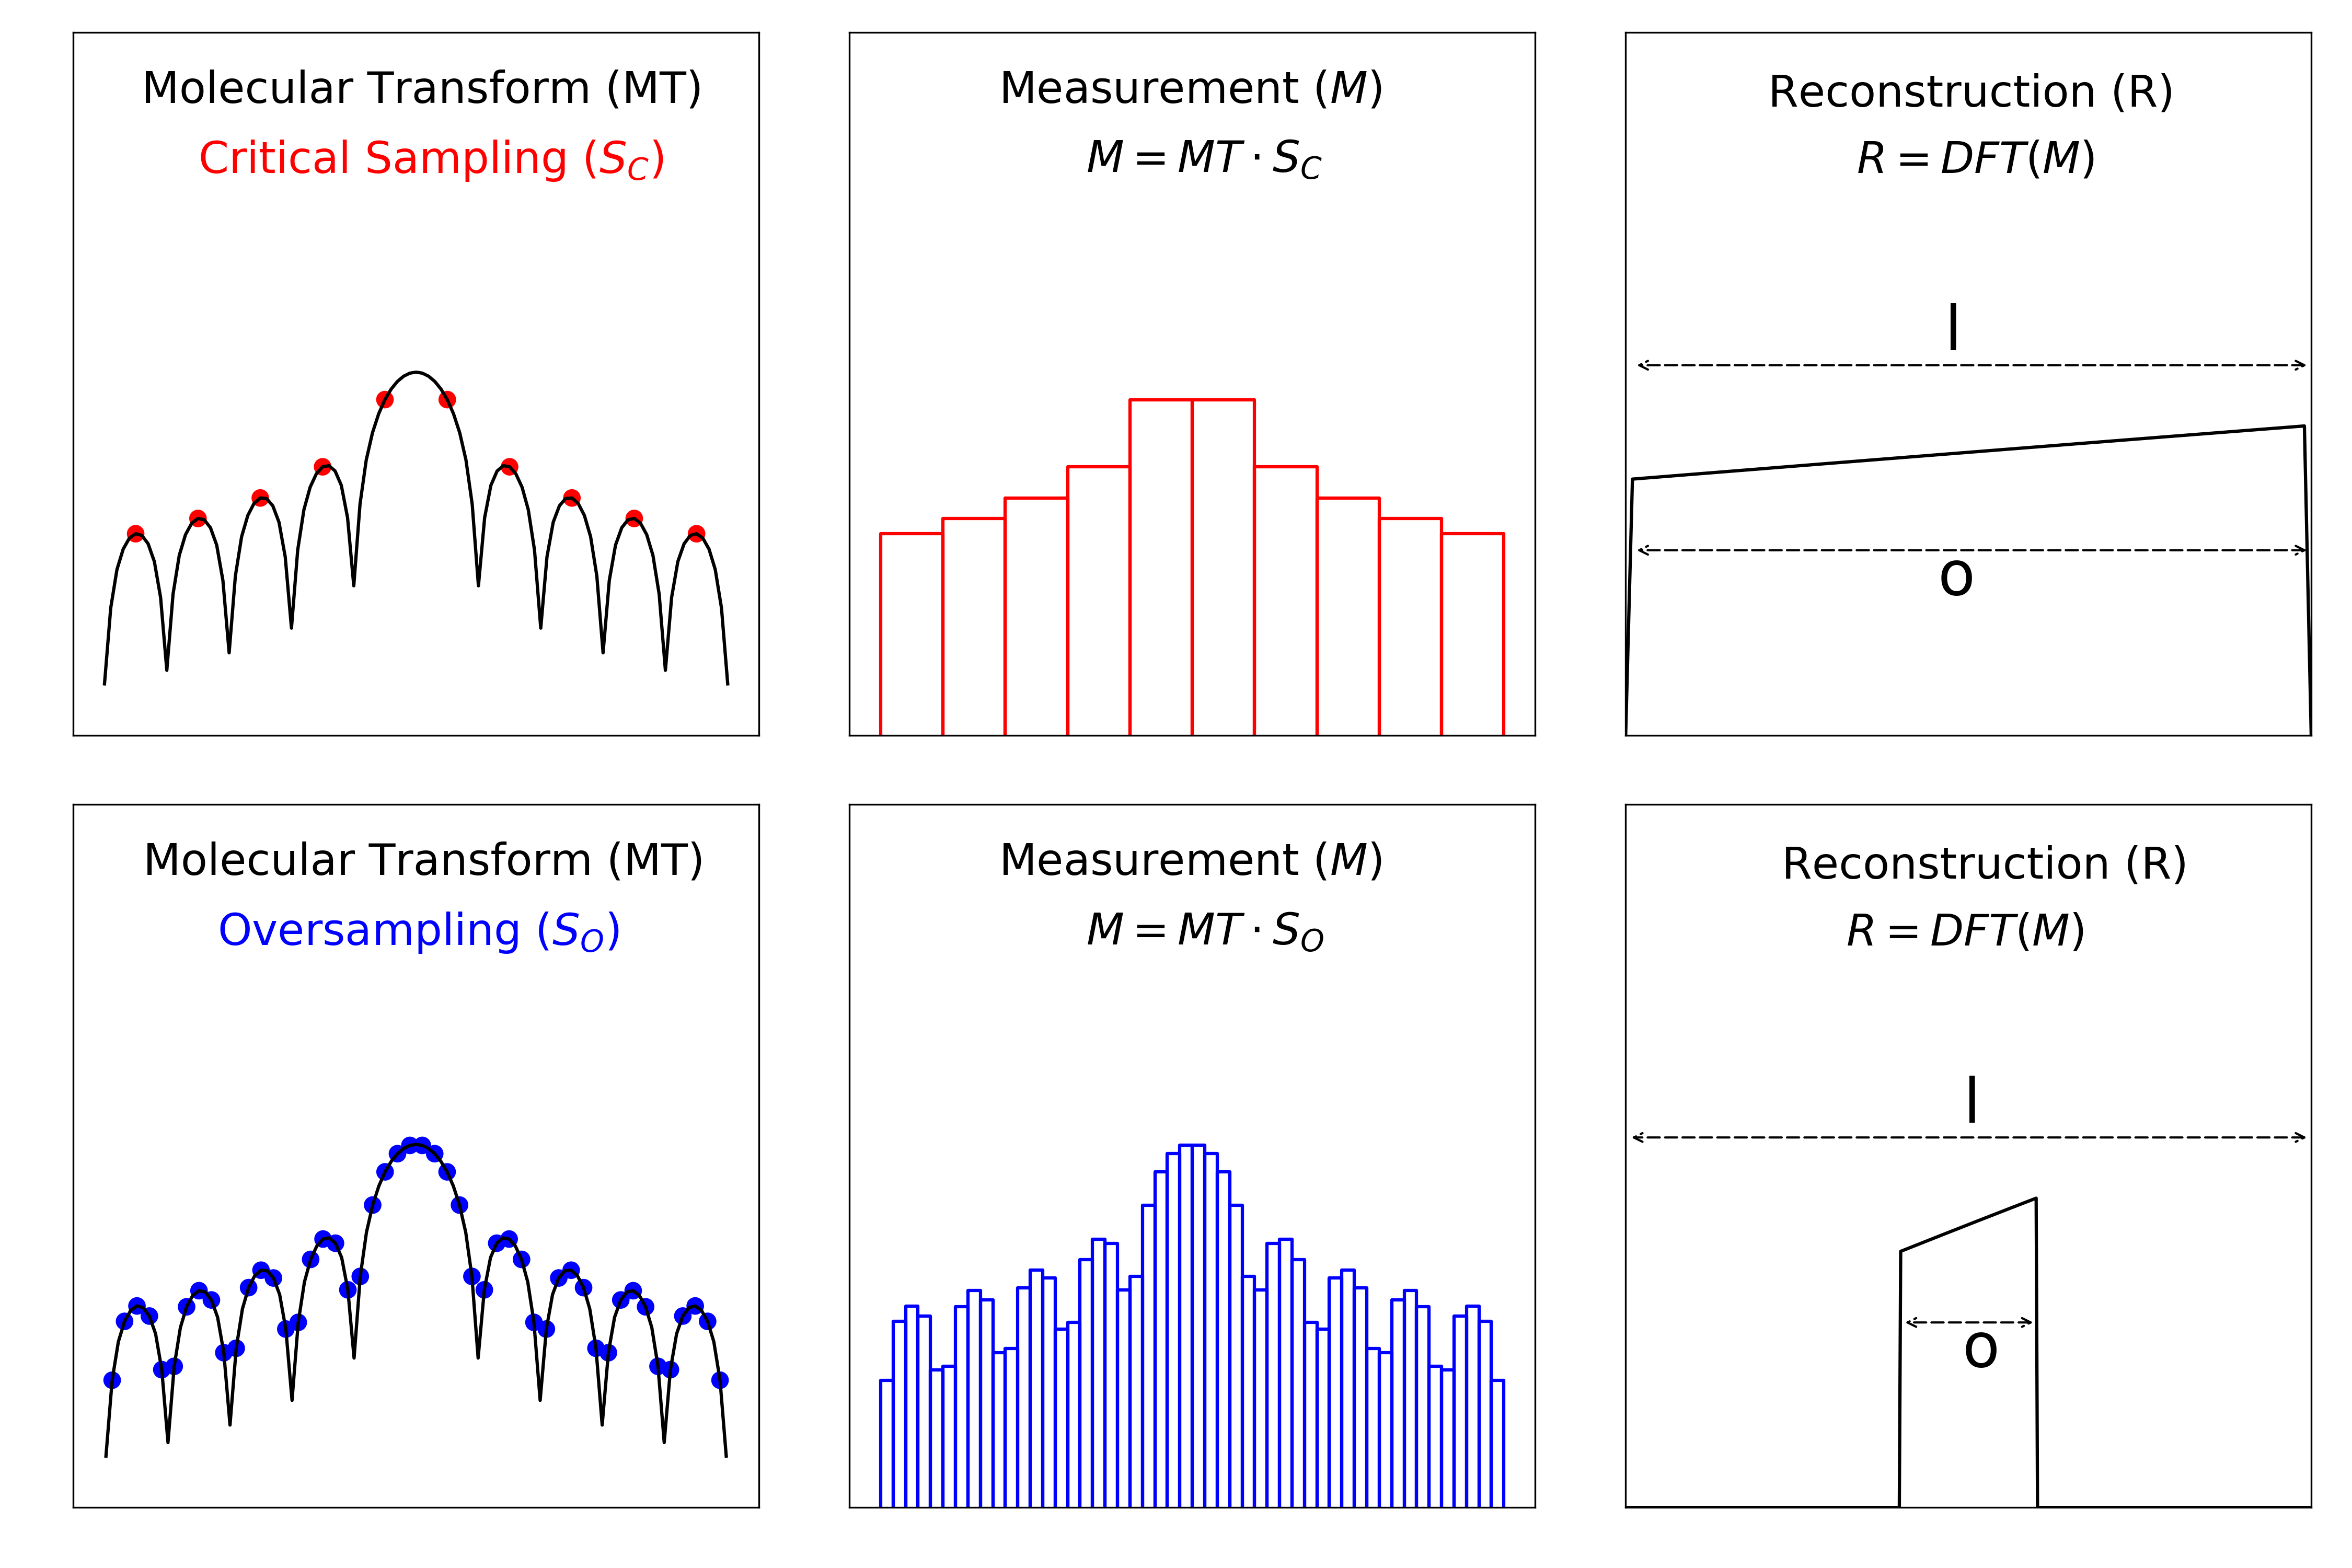
\includegraphics[width=120mm]{sampling.png}
	\caption{Illustration of critical sampling versus 		oversampling.}
	\label{fig:sampling}
\end{figure}

By choosing a detector setup such that the sampling rate is at least twice the critical sampling rate we can, in some cases, use the additional intensity information to recover the phases, and thus reconstruct the object from the measured intensities alone. It is known that this method does often does have multiple solutions in 1D \cite{Walther1963}, however, for higher dimensions it has been proven that, in most cases, an oversampled pattern will have a unique solution\cite{Bruck1979}. Oversampling is the basis of many phase retrieval techniques in SPI, as well as some clever phasing techniques in SFX \cite{Ayyer2016,Chapman2011}.

\section{Iterative Phase retrieval}
In practice there are many ways of actually retrieving the phase information from the diffraction pattern, but most common phase retrieval techniques are variations of convex optimization algorithms. This section introduces the general idea behind convex optimization, and explains the working three different algorithms. It has to be appreciated that solving the phases problem in remarkably difficult, as it is neither linear nor convex.

As with any difficult problem, one starts from the things that are known. Figure \ref{fig:sampling} shows that oversampling in Fourier space implies that there is an area the size of ($l-o$) around the object for which we know the electron density $\rho(\vec{r})$ is zero. This knowledge can be used as a constraint on the possible phases: we know that a correct choice of phases would make the corresponding $\rho(r)$ be zero in this area. The area that can contain positive electron density is called the support mask $M(\vec{r})$. This constraint is called the real-space constraint. Furthermore, we know that the recovered Fourier amplitudes should agree with the measured intensities. This is called the Fourier-space constraint. 

In 1978 Fienup \cite{Fienup1978}, inspired by an earlier algorithm by Gerchberg and Saxton [Gerchberg1972], introduced an algorithm called Error Reduction (ER) to solve the phase problem. ER is an iterative approach that tries to find the solution that minimizes the disagreement to both the real-space constraint and the Fourier constraint. In words it can be described as follows:\\
\begin{enumerate}
\item Assign random phases to each pixel.
\item Inverse Fourier transform F(s).
\item Set all electron density outside of $M$ to zero, keep other electron density.
\item Fourier transform $\rho(r)$
\item Make sure that the recovered amplitudes match the measured intensities. Keep the phases.
\item Go back to step 2.\\
\end{enumerate}


ER is sometimes able to find the correct solution, but because the problem is not convex, in general it often gets stuck in local minima, making ER unable to find the global solution.

In 1984 Levi and Stark realized that applying the above described constraints can be interpreted as projections in a multidimensional Hilbert space \cite{Stark1984}. Step 3 will from now on will be called the real-space projection $P_r$. A combination of step 4,5 and 2 will be called the Fourier Projection $P_f$.  In ER $P_r$ and $P_f$ can be defined as follows:
\begin{align}\label{eq:ER}
P_r \rho\left(\vec{r}\right) =& \begin{cases} \rho\left(\vec{r}\right) \quad &\mathrm{if}\,\,
    \vec{r} \in M\\0 \quad & \mathrm{if}\,\, \vec{r} \not\in M \end{cases}\\
P_f \rho(\vec{r}) =& \mathcal{F}^{-1}\left( \frac{\sqrt{I}}{|\mathcal{F}(\rho(\vec{r}))|}\mathcal{F}(\rho(\vec{r})) \right)
\end{align}

The largest difference between both projections is that the support constraint is convex, while the Fourier constraint is not. An iteration in ER can now been seen as a real-space projection followed by a Fourier projection. This can be summarized as:
\begin{equation}
\rho_{n+1}\left(\vec{r}\right) = \begin{cases} P_f\rho_{n}\left(\vec{r}\right) \quad &\mathrm{if}\,\,
    \vec{r} \in M\\0 \quad & \mathrm{if}\,\, \vec{r} \not\in M \end{cases}
\end{equation}

Two error metrics can be associated with both projection;the fourier error ($E_f$) and the real space error ($E_r$). $E_r$ is the fraction of density outside the support. $E_f$ shows the difference between the recovered amplitudes and the square root of the intensities. Mathematically $E_f$ and $E_r$ are defined as:

\begin{equation}
E_r = \left|P_r\rho(\vec{r}) - \rho(\vec{r})\right| = \left(\sum_i\rho_i^2\right)^{\frac{1}{2}}
\end{equation}

\begin{equation}
E_f = \left|P_f\rho(\vec{r}) - \rho(\vec{r})\right| = \left(\sum_{i}\left(\frac{\sqrt{I_i}}{|F(S_i)|}- F(S_i)\right)\right)^{\frac{1}{2}}
\end{equation}
  
\subsection{The Hybrid Input Output algorithm (HIO)}
In 1982 Fienup introduced an algorithm that can escape from local minima, the so-called the Hybrid Input Output algorithm (HIO). To achieve this HIO makes use of a so called relaxation parameter $\beta$. An iteration in HIO can be described as follows:
\begin{align}
\rho_{n+1}\left(\vec{r}\right) = \begin{cases} P_f \rho_{n}\left(\vec{r}\right) \quad &\mathrm{if}\,\,
    \vec{r} \in M\\\rho_n(\vec{r}) -\beta P_f \rho_n(\vec{r}) \quad & \mathrm{if}\,\, \vec{r} \not\in M \end{cases}
\end{align}

I see the $\beta$ parameter similar to temperature in simulated annealing. If $\beta$ is large even deep local minima can be escaped. Unfortunately this also means the global minima might be missed as well. If beta is small HIO will miss fewer minima, but will have greater difficulty escaping from them. As long as a minimum is not perfect ($E_r$ and $E_f$ are not both zero), HIO will, however, eventually be able to escape \cite{Martin2010}.

\subsection{The Relaxed Averaged Alternating Reflection algorithm (RAAR)}
Another algorithm that is used often in the work described in this thesis is the Relaxed Averaged Alternating Reflection algorithm (RAAR). RAAR does not escape all minima but it can escape shallower once. For high-quality data RAAR seems to find the solution quicker than HIO, and also in a more behaved manner. An iteration of RAAR can be described as follows:
\begin{align}
\rho_{n+1}\left(\vec{r}\right) = \begin{cases} P_f \rho_{n}\left(\vec{r}\right) \quad & \mathrm{if} \,\,
    \vec{r} \in M\,\mathrm{and}\,\rho_n(\vec{r}) \geq -(1+\beta)P_f\rho_n(\vec{r}) \\\
    \beta\,\rho_n(\vec{r}) -(1-2\beta) P_f \rho_n(\vec{r}) \quad & \mathrm{if}\,\, \mathrm{otherwise} \end{cases}
\end{align}

As both RAAR and HIO do not guarantee to end up in the bottom of a minimum, concluding phase recovery with a number of iteration of ER will ensure the bottom of the final minimum is found. This can improve the overall quality of the reconstruction, as shown in \textbf{Paper I}.

\subsection{Other algorithms}
There exist many other phase recovery algorithms. Examples are: diffusion map (DM) \cite{Elser}, GHIO[], HPR [], HAAR[] , ESPRESSO [], saddepoint optimisation [], and charge flipping []. A software package called Hawk allows users to select and test different algorithms. Hawk is especially powerful as it gives graphical feedback of the reconstruction process. This can for example be very useful to find the correct support size. 

\section{Validation}
In iterative phase retrieval every reconstruction results in an image, irrespective of it having biological relevance or not. It is therefore very important to have tools to validate a reconstruction. This section will describe different validation tools used in the field.

\subsection{Errors}
The most basic method to assess the difference in quality between two reconstructions is comparing the respective errors. The reconstruction with lower errors is generally considered to be a more successful reconstruction. This method however does not tell anything about the biological validity of a reconstruction and is most often only used to exclude outliers (reconstructions that have clearly failed).
 
\subsection{PRTF}
The standard tool to assess the quality of a reconstruction is the phase retrieval transfer function (PRTF). This function considers the variation within a set of independent reconstructions (each reconstruction starting from a random set of phases), and uses this variation to quantify the resolution of a reconstruction. The basic assumption behind the method is that if a similar object is retrieved repeatedly, this object is supposed to be similar to the true object. The variation between reconstructions is calculated for each pixel $i$ by adding all recovered amplitudes for that pixel and dividing the total vector by square root of the measured intensity for that pixel $v_i = |\frac{\sum A_i}{\sqrt{I_i}}|$. If the value of $v_i$ is close to unity all reconstructions recovered a similar amplitude for pixel i. The closer $v_i$ is to zero the more difference there is between individual reconstructions. The standard PRTF plot shows the radial average of $v_i$. A common practice is the field is to define the resolution of a reconstruction as the first time the 1D PRTF drops below $\frac{1}{e}$. This threshold is arbitrary. For spherical objects a periodic drop in the 1D PRTF, corresponding to a drop in measured intensity, can be observed. This drop can be explained by the fact that the phase of a pixel measuring 0 intensity is unconstrained.
 
\subsection{Missing Mode Analysis}
As described in previous sections diffraction patterns lack data. Even in the best case the central region will be missing because the direct beam will otherwise damage the detector. The main other sources of missing data are detector geometry and saturation. 

Reconstruction algorithms deal with this missing data by recovering the phase as well as the amplitude for the pixels in these regions. In many cases the missing data does not affect the stability of phase recovery, however this cannot be said in general. For this we have to note that the Fourier constraint does not limit the amplitudes in the missing data area, and the real-space constraint does not limit the electron density inside the support. If there exists an object that can fit inside the support and has a Fourier transform that is zero outside the missing data region, this object could be arbitrarily added to the solution and thus would form an ambiguity in the reconstruction process.

In general completely unconstrained objects do not exist. Objects that fit the support constraint and only slightly contribute outside the missing data region, i.e. weakly constrained objects, can however exist. In the design of an experiment, or when deciding whether or not to phase an object it is important to have a tool that predicts whether weakly constrained objects exist or not. Missing mode analysis is such a tool.

The DFT can be represented in matrix form, where each column represents a pixel in real space and each row represents a pixel in Fourier space. The rows and columns can be reordered according to whether they conform to the fourier and real space constraints or not.

\begin{equation}\label{equ:F_split}
  \mathcal{F} = 
  \left(\begin{array}{l|lll}
    \mathcal{F}_{SM} & &\mathcal{F}_{\bar{S}M}& \\\hline
    &&&\\
    \mathcal{F}_{S\bar{M}} & & \mathcal{F}_{\bar{S}\bar{M}} &\\
    &&&
  \end{array}\right)
\end{equation}

We are after objects that minimize $|\mathcal{F}_{SM}\rho|$. A common method to find such objects is singular value decomposition [Eckart]. This method decomposes $|\mathcal{F}_{SM}\rho|$ into a diagonal matrix $\Sigma$, and two unitary matrices U and V in the following way.

EXPLAIN EIGENVALUES AND BASIS




\subsection{Hierarchical clustering}
To test whether the Fourier Error and Real space error are good measures to assess the variance between individual reconstructions, a clustering analysis can be performed. An example of such an analysis is UPGMA (Unweighted Pair Group Method with Arithmetic Mean) hierarchical clustering [Sokal, Michener]. This method checks the similarity between reconstructions by making pairwise pixel-to-pixel comparisons between all reconstructions. The similarity score is the normalized scalar product between a pair reconstructions after translating them to their optimal fit. We plot the similarity score of  each cluster as a function of the number of clusters and choose the agglomeration step where the plot makes a "kink". This is a standard way to estimate the number of clusters present in the set of reconstructions. This capability is an advantage of the UPGMA clustering algorithm. In a 2D plot of FE vs RE, color-coded by cluster, it is possible to see whether or not there is a correlation of reconstruction similarity and error score. An illustration of this method can be found in \ref{fig:UPGMA}
 
\begin{figure}[h]
	\centering 
		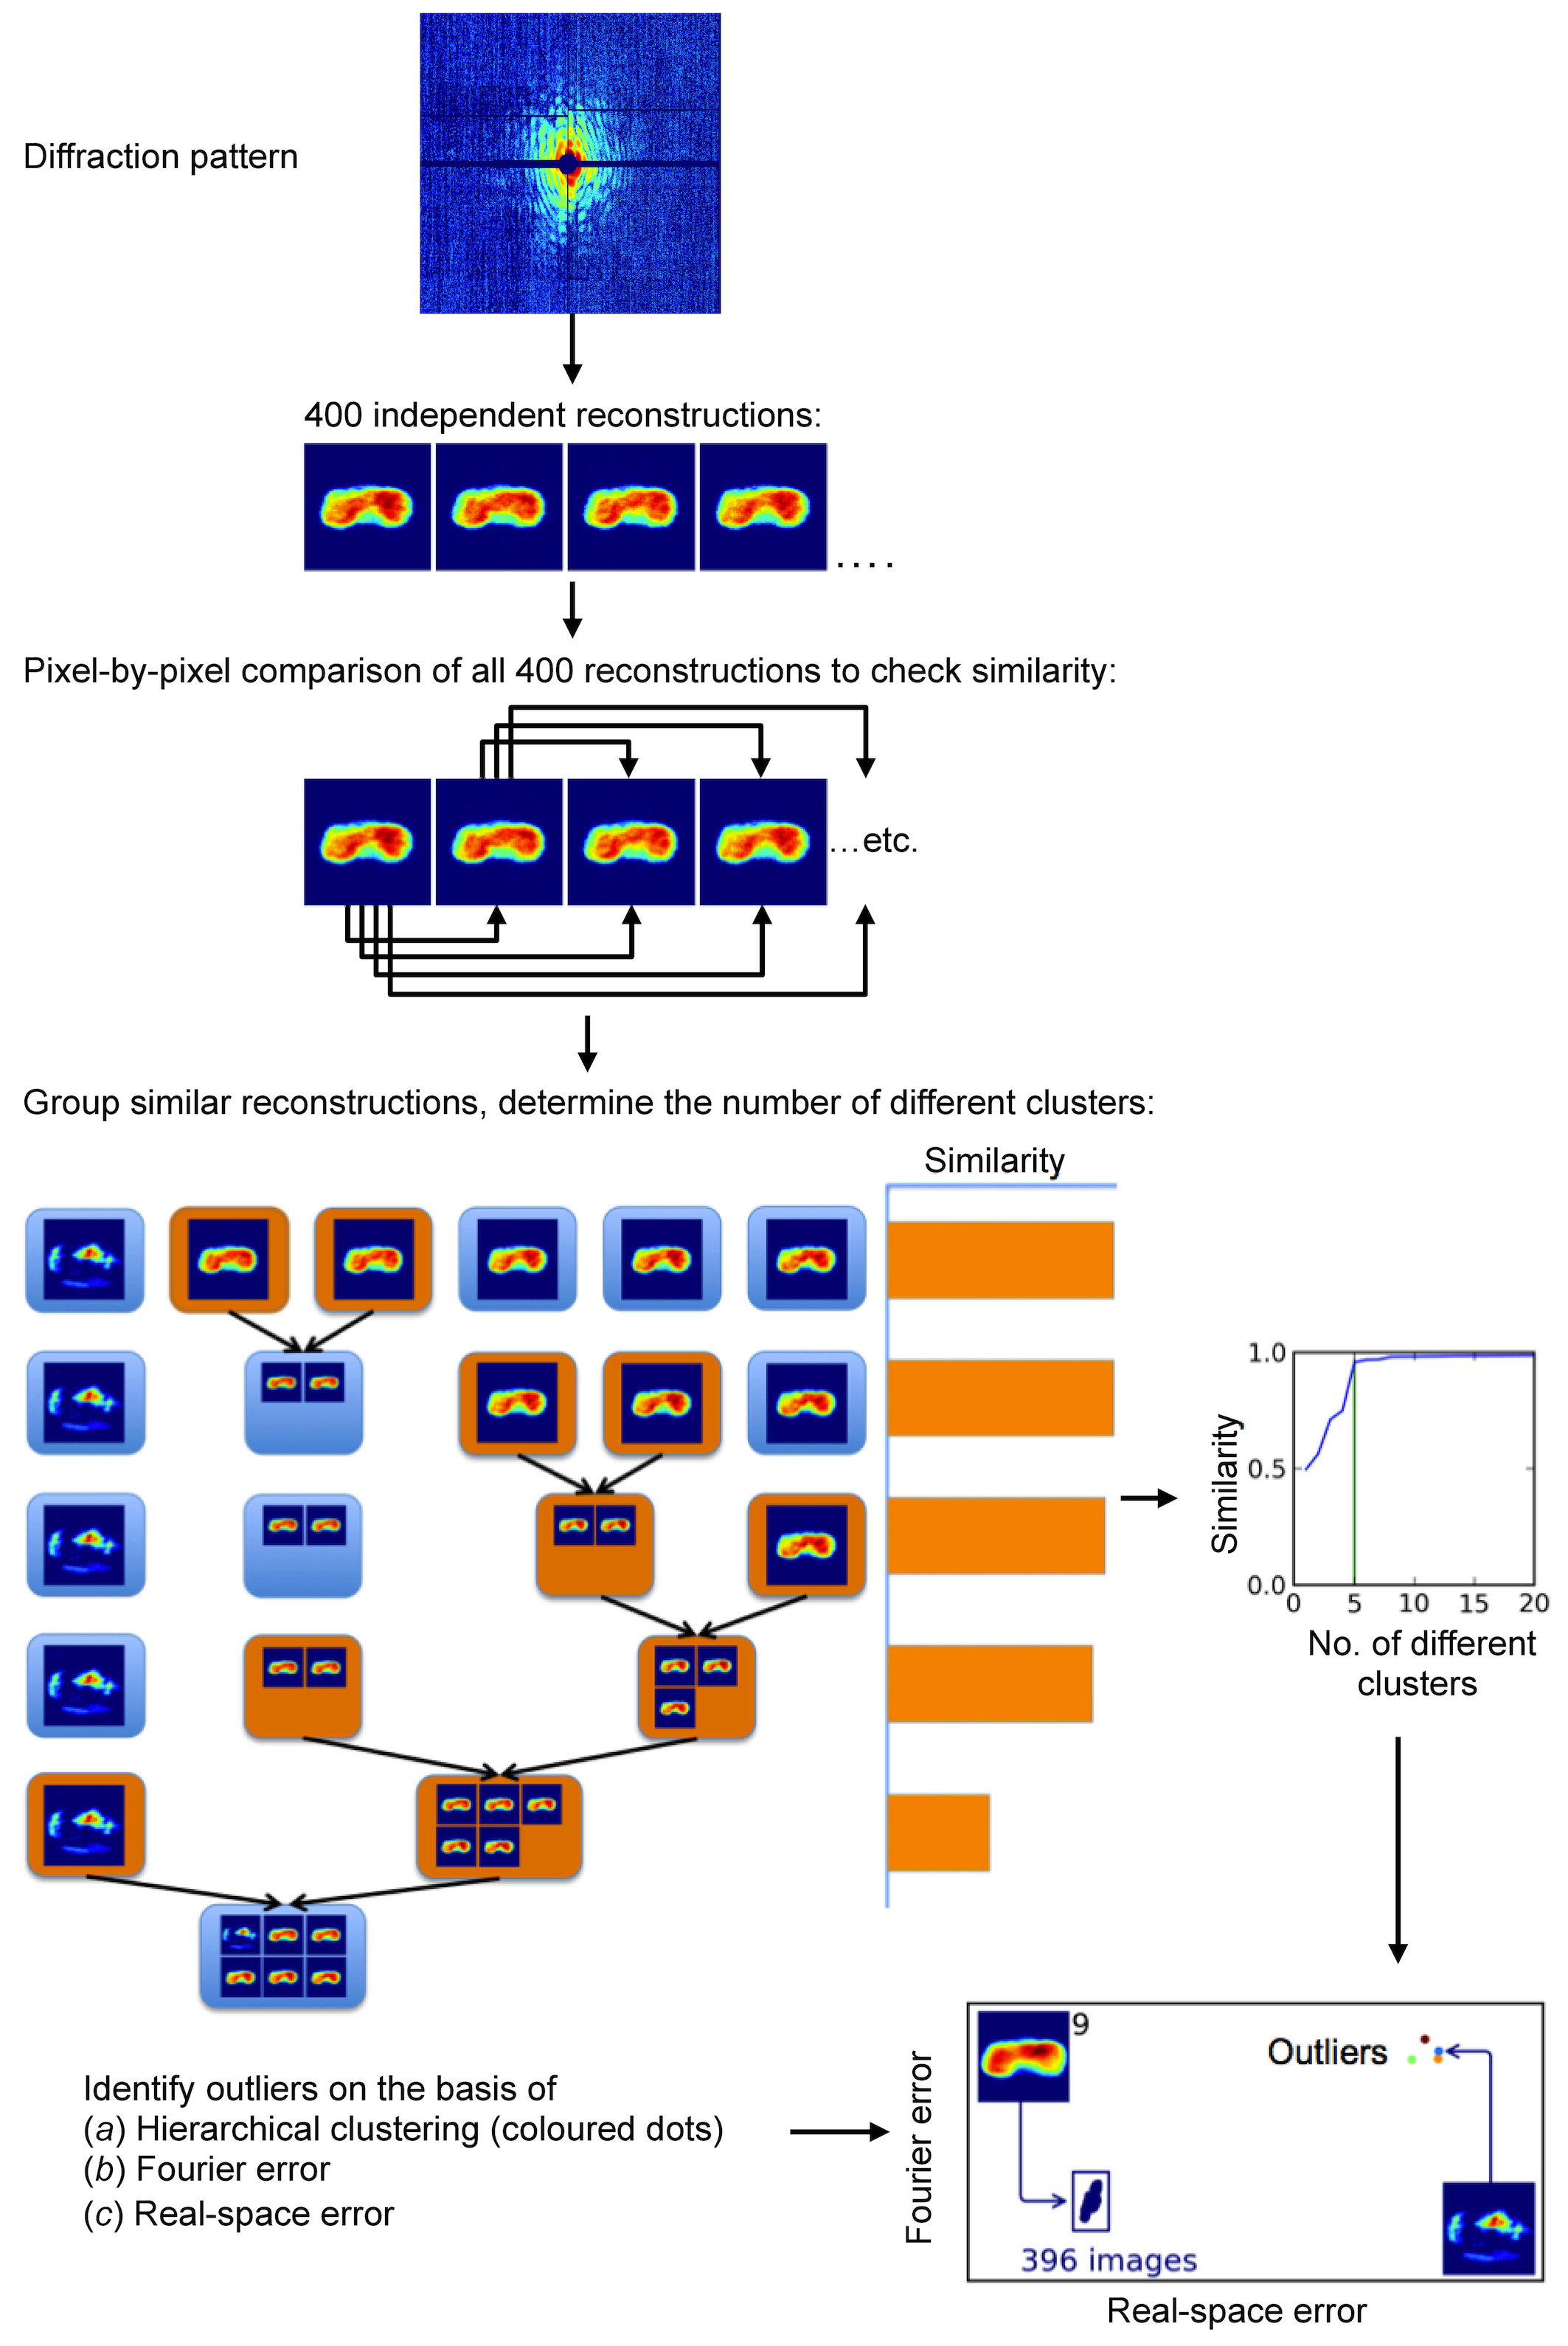
\includegraphics[width=100mm]{UPGMA_Clustering.jpg}
	\caption{UPGMA Clustering.}
	\label{fig:UPGMA}
\end{figure}

In the case that several large clusters remaining after applying a real-space error and Fourier-error threshold the clusters have to be examined carefully. If the remaining clusters correlate with the errors we suggest to keep only the cluster with the lowest error. If no correlation is present between score and cluster it is advised to keep all clusters for further evaluation. Otherwise there is a possibility of selecting on similarity, which would negate the validation power of the PRTF.

 
\section{Simulated Phase Contrast Methods}
Once one has retrieved the phase of the diffraction pattern, one has complete knowledge of the information encoded in the said wave-field. This total knowledge is powerful, because it allows the emulation of the action of any imaging system for which an associated mathematical transform can be written, regardless of whether that system is experimentally realizable in hardware.

For example, differential interference contrast imaging or Nomarski imaging is experimentally a well established technique to visualize the changes in phase. This change can have biological meaning, as for example the density inside certain organelles can be higher than the average density in cells. Normarski imaging will give a more pronounced image of the borders of the organelle. For an example see ref [mitochondrium). 

Nomarkski imaging in its simplest form takes a coherent wave-field of interest, say $\psi(x,y,z = 0)$, and then interferes this wave-field with a copy of itself that has been given both a slight transverse displacement ($\Delta x$, $\Delta y$) and a phase shift $\phi_0$ (Nomarski and Weill,1955). Thus the intensity of the resulting wave-field is [Paganin]:
$|\psi(x,y,z=0)+ e^{(i\phi_0)} \psi(x - \Delta x,y - \Delta y,z=0) |^2$, from which one can show (using the Fourier shift theorem) that the transfer function becomes:
\begin{equation}
\begin{aligned}
\begin{split}
T_{DIC}(k_x, k_y, \tau) = 1 + e^{(i(\phi_0 - k_x \Delta x - k_y \Delta y))},\\
\tau = (\phi_0, \Delta x, \Delta y)
\end{split}
\end{aligned}
\end{equation}

In the case of a reconstructed image $\rho(\vec{r})$, the Normarski variant will look like:
\begin{equation}
N = \mathcal{F}^{-1} T_{DIC} \mathcal{F}(\rho(\vec{r}))
\end{equation}
We have created simulated Nomarski images of the reconstructed cell images shown in the results part.

\section{Shrinkwrap}
While HIO and RAAR perform well when the support is tight and well known, phasing can practically become impossible if the support is too large. In 2003 Marchesini developed an algorithm that does not require a priori known support as input, but instead tries to deduce the shape of the support during the reconstruction. It starts by guessing the support from the autocorrelation. It does so by blurring the autocorrelation and selecting all pixels above a certain threshold to be included in the support. Consecutively after each n iterations the support is updated by applying a Gaussian blur to the real space image and selecting the pixels that have a value above a certain threshold. By varying the amount of blur and/or the selection threshold as the iterations progress, the support can slowly wrap and shrink to the true shape of the object. The general idea behind the algorithm is that even with a non-accurate support some features will be recovered well, and by using these features finally the an accurate support will be found. The algorithm has been very successful for experimental data [].

\chapter{3D restructions}
So far we have dealt with 2D diffraction patterns. Although much can be learned (and has been learned) from 2D images, having a structural 3D model is essential to understand the functioning of biomolecules. From the Fourier slice theorem we know that a diffraction pattern is a 2D slice through the center of the 3D diffraction pattern of the object. Different slices could therefore build up the 3D fourier transform of the object. In the current CXI setup it is impossible to image one object multiple times, making it difficult to reconstruct the complete 3D diffraction volume from one particle alone. If the particle of interest is reproducible the diffraction pattern from each copy could be used to construct the 3D fourier transform of the object. This does pose a new problem: the relative orientation of each diffraction pattern compared to the others has to be recovered. A variety of reconstruction algorithms have been proposed for recovering the relative orientation of diffraction data, including the EMC algorithm [Loh], the manifold embedding algorithms [Giannakis], simple best-fit models [Tegze], and multi-particle cross-correlation analysis [Saldin, Kirian, Kam, Kurta]. Theoretical studies suggest that the determination of diffraction pattern orientation should be possible even with very low photon counts of as little as 1000 scattered photons per image [Loh], making EMC and ME very suitable to recover the 3D structure of sparsely scattering single proteins.

\section{the EMC algorithm}
The EMC algorithm is an iterative program. On the one side you have the 2D measured intensity patterns ($IM_i$), and on the other side a 3D model of the Fourier space of the object ($M$). Each iteration starts with the expand step in which the 3D model is expanded in n central 2D slices ($IP_i$). N is dependent on the sampling rate of the 3D model. Each of the slices are compared to each diffraction pattern, using a model for the noise, to predict a probability score that the measured diffraction pattern is coming from the model diffraction pattern. To paraphrase: imagine that you would image each particle at the same orientation, the measured diffraction patterns will not be identical, since the noise is varying from shot to shot. Each pixel however will have an associated distribution of measured intensity values. Based on this distribution, which can for example be Poissonian in the case of pure shot noise, one can assign a probability that $IM_i$ is coming from slice $IP_i$. In  a good model not only will the measured values for a given 3D pixel (voxel) be similar for different $IM$, the distribution of measured values will have to be similar to the known noise distribution. This is a very subtle idea and utilizes the data very efficiently.

Comparing all $IM_i$ to each $IP_i$, lead to n probability distributions predicting the likelihood of the orientation of the measured diffraction patterns. This step is called the maximize step. Using the probability distributions as weights, a new model $M_{n+1}$ is generated from the measured diffraction patterns in the so-called compress step. 
The initial model $M_0$ can be a random model. After one iteration a similar patterns will end up in similar orientations which hopefully will make $M_1$ a bit more similar to the real Fourier pattern of the particle. After repeating this Expand-Maximize-Compress cycle multiple times a realistic model might be generated.

\section{Non-reproducible objects}
The addition of diffraction patterns from non reproducible object (i.e. incoherent addition) is very problematic in Fourier space space [Maia], as all features of the resolution of variation will be washed out. This makes it very difficult to retrieve 3D information from an heterogeneous object such as cells and the fold of many proteins. The tackle the heterogeneity problem many adaptations of existing algorithms or new algorithms have been developed.

\subsection{Multi-model EMC}
Currently a version of EMC is on its way that can generate multiple models of the same particle. It is very similar to single state EMC, but differs in the fact that it build multiple self-consistent models. 

\section{the Manifold Embedding algorithm}


\subsection{Tomography and sub-tomogram averaging}
Tomography used a set-up in which the object is imaged from m different but known orientations. Sometimes this is enough to gain enough information about the object in 3D. Crowther's criterion describes the relation between resolution and number of required exposures (m). For large objects and/or high resolutions it becomes difficult to have enough exposures to recover the full object at atomic resolution. In this case one could use multiple low resolution parts of the tomogram (sub-tomogram) to build up a model of semi-repoducible object in a method similar to EMC. The limit of the number of beams (m) for which this is possible in an XFEL setup is currently under investigation.

\subsection{Holography}
At high resolutions the detector does not measure the Ewald sphere and the Friedel symmetry of the diffraction pattern breaks. This is often very visible at longer wavelengths (<400 eV). This curvature can be exploited to resolve semi-3D information about the object, but the extend at which this is possible is disputed. In some cases much is known about the possible shape or buildup of the particle and then it is possible to reconstruct a 3D structure [Miao, Fennel, ...]

\chapter{Image Classification}
In order for algorithms such as EMC to work, the amount of heterogeneity within the diffraction data set has to be limited [TOMAS is there an article describing this?]. Furthermore, each of the steps in the experiment introduces it own type of noise to the measured diffraction pattern. For example think of the debris clumping around small particles compared to the drop when sprayed with the GDVN, detector malfunctioning or saturation, or intensity fluctuations due to the random start of the SASE process. Often the results of the first two types of noise can not be tolerated by EMC, and image classification before the EMC step is necessary. Also fast feedback about the first type of noise is very useful to have during the experiment. So far a very robust sizing method has been developed, but more extended methods might come in useful. Several methods shown here can give rapid feedback on the heterogeneity of the particle.

\section{Template-based classification}
If your object has a known shape it could be possible to only select the diffraction patterns that are similar to a set of expected diffraction patterns from the object called templates. Paper III explores the possibility of template-based classification. In general this method is highly dependent on the choice of template, as well as the amount and type of variation present in your sample.

\section{Feature extraction}
Another way of selecting diffraction patterns is by extracting general features from the diffraction pattern such as size, particle shape, amount of saturation, number of particles in the beam. Based on the relative values associated with the features patterns might be selected or not, or the experimental conditions might be rapidly adjusted. This section describes several methods to extract features.

\subsection{Size}
A common method to determine the size of an object is fitting the central speckle to the central speckle of simulated diffraction pattern from a sphere. This method has shown to be successful for particles that have an icosahedral shape to spherical shape \cite{Hantke2014,Daurer2017}. If the diffraction pattern also has the 3rd to the 5th minima present, the average of these minima can also be used to describe the size of the object. This method might be especially useful for strong scatterers, because the central speckle or first minimum might not be reliable due to saturation effects.

It might also be possible to determine the size and shape of an object from a filtered autocorrelation. This is useful when the object cannot be approximated by a sphere, but is rather elongated in one axis. Due to aerosol injection, the strongest contrast in the object is coming from the edge of the object. Therefore the edge is often one of the most clear features in an autocorrelation. This method is limited to convex objects.

\subsection{Multiple scatterers in the focus}


\subsection{Edge detection}
Some objects are characterized by having sharp edges. A sharp edge in real space corresponds to a streak in the direction perpendicular to the edge in Fourier space. Objects and/or orientations of objects might be classified by determining if streaks are present, and how many. Figure explains the idea behind a streak finding algorithm described in paper IV.


\chapter{Software}
\section{RedFlamingo}

    \part{Results}
\chapter{Results}
\section{Imaging live cells}
For the study described in paper I we used cells of two species of cyanobacteria as a sample (Cyanobium gracile and Synechococcus elongatus). Cyanobacteria are photosynthetic bacteria that can be found in almost any habitat on earth, ranging from hot volcanic areas to cold polar ice caps. They play an important role in the global carbon cycle. In a 25 day cycle an algal bloom of 1000 $km^2$ can sequester around 22,000 tonnes of atmospheric carbon into organic carbon before cyanophages caused the bloom to collapse.
 
Cyanobium gracile cells were selected for their small size, their robustness with respect to the injection procedure, and convenient autofluorenscence properties to assess cell viability. Solitary C. gracile and S. elongatus cells have an oval-to-cylindrical shape, and vary in size between 0.25-0.4 $\mu$m in diameter and 0.4-4.0 $\mu$m in length [Komarek]. Cell divide symmetrically by binary fission. The two daughter cells separate from each other after reaching the size and shape of the mother cell [Komarek2]. We used non-synchronised cell cultures undergoing active growth providing cells in various stages of their cell cycle. 

The experiments described in paper I was carried out at the atomic, molecular, and optical science (AMO) endstation at LCLS at 512 eV (2.40 nm) and 1100 eV (1.13 nm) photon energy.  Figure \ref{fig:ExperimentalSetup} shows the arrangement of the experiment. The length of the photon bunch was about 70 fs. The pulse was focused to a spot of 3 $\mu m$ x 7 $\mu m$. The average photon density in the focus was about $1.1 x 10^{11}$ photons/pulse/$\mu m^2$ at 517 eV, and $8.6 x 10^{10}$ photons/pulse/$\mu m^2$ at 1,100 eV. Far-field diffraction patterns were recorded on a pair of pnCCD detectors [Struder] in the CFEL-ASG Multi Purpose (CAMP) instrument [Struder]. The detectors were place at 741 mm downstream from the interaction region of the beam and the sample. The detector read out rate matched the 120 Hz repetition rate of the LCLS. 
\begin{figure}[h]\label{fig:ExperimentalSetup}
\centering 
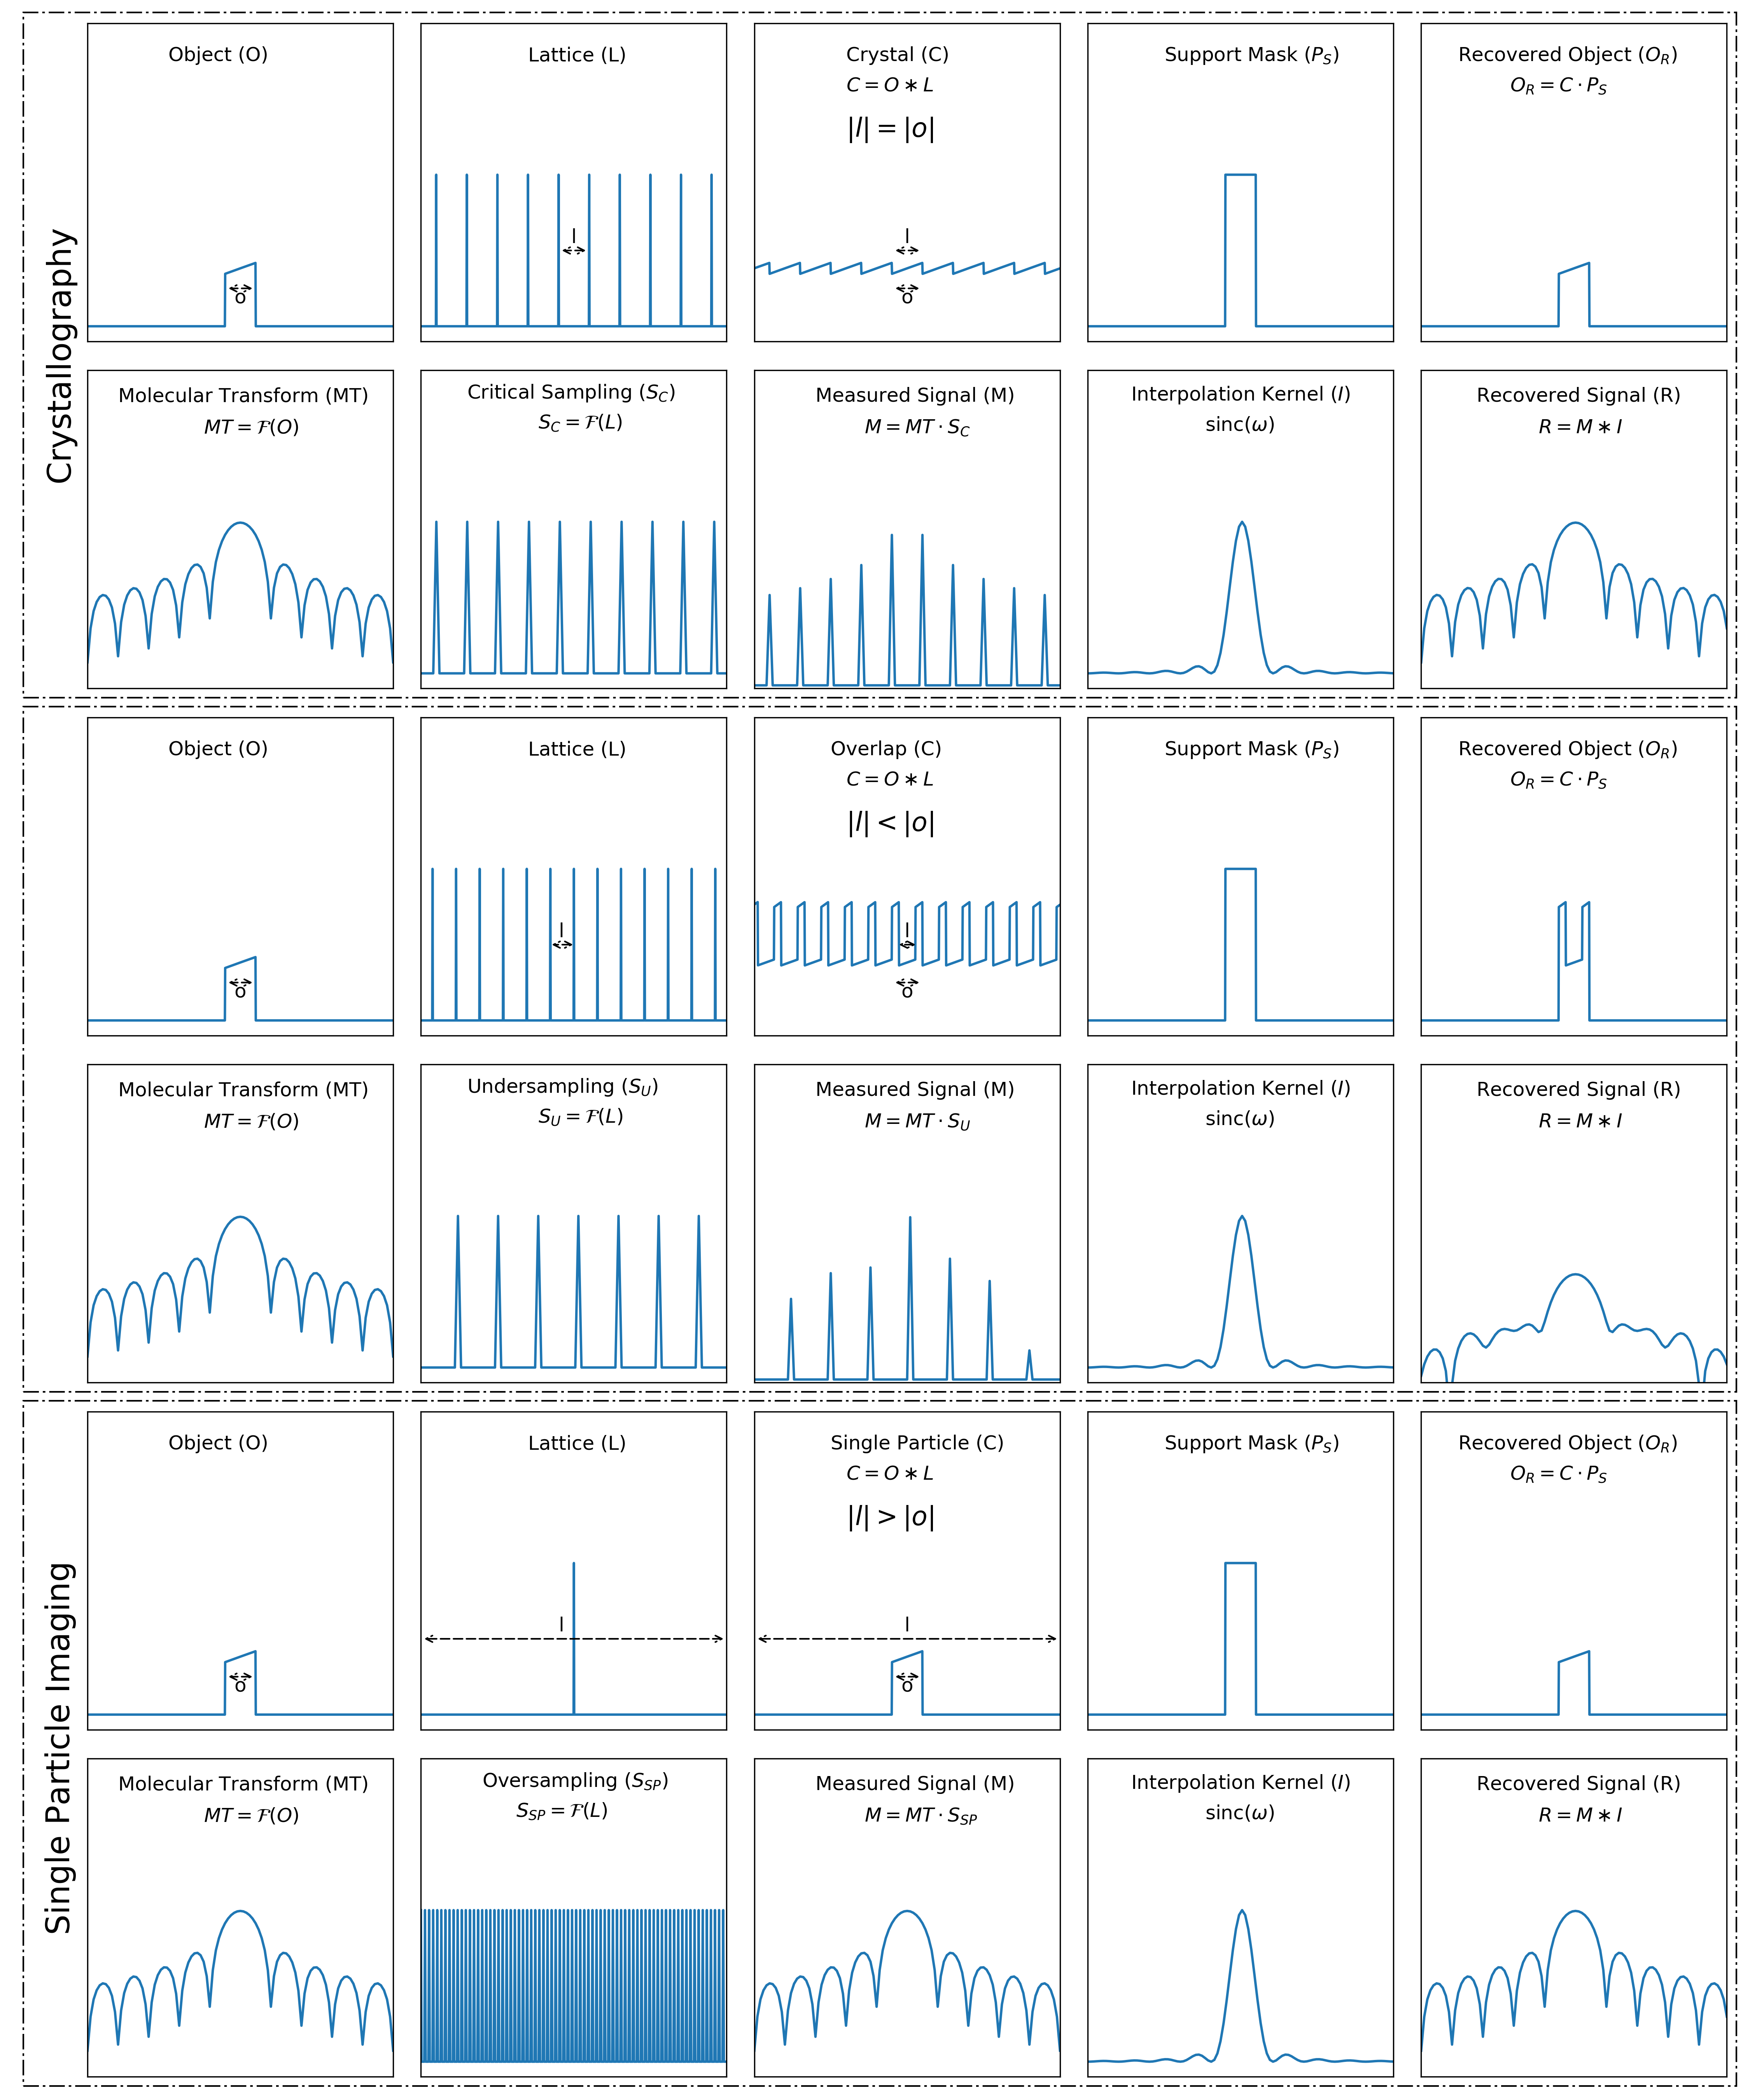
\includegraphics[width=120mm]{SamplingTheory.png}
\caption{Different rates of sampling explained}
\end{figure} 

We collected diffraction patterns of C. gracile cells for 60 minutes at a hit ratio of 43\% and selected the 7,500 clear single hits for further analysis, using the Cheetah software package. The oversampling rate of the particle was around 12-fold, which allowed direct phase recovery from the measured intensity patterns. This was not a trivial problem because strong hits saturate the detectors at low diffraction angles. As a compromise, we selected medium-strong hits, which contained either no, or only few saturated pixels while still providing scattered signal to reasonably high resolution. Missing mode analysis revealed no unconstrained modes for all cells presented in paper I. 

Figure 2 a-j shows the reconstructed exit wave-fronts (images) for ten live C. gracile cells together with the corresponding diffraction patterns, and a synthetic DIC image. The reconstructions represent 2D projections of the electron density of the cells. The images are arranged by increasing size, and show the expected morphologies of cells during division [Komarek,Komarek2]. The resolution of each  reconstruction is indicated by the size of the round white dot. Features smaller than the dot need to be interpreted with care.

Phases were retrieved using the Hawk software package. For each pattern 400 reconstructions were made, each starting from different random initial phases. These reconstructions consisted of 5000 iterations with the RAAR algorithm [Luke], using a Shrinkwrap algorithm[Machesini] for support determination, and concluded with 100 iterations by the ER algorithm[Fienup, Gerchberg-Saxton]. The initial and final support size was selected manually. No additional constraints were used since we anticipated the effects of absorption in the thick cells to give effects similar to a phase object. 

Resolution for the reconstructions was estimated from the PRTF (See Figure \ref{fig:ExperimentalSetup}), using the 1/e cutoff. Before calculating a PRTF and averaging the images we removed outliers among the reconstructions by applying a threshold to the Fourier error. Clustering validates the results from using a threshold on the Fourier-Error and the real-space error(Figures 7 a-j). On average the main cluster contained about 370 out of 400 reconstructions (93), except for one case where only 96 reconstructions formed the biggest cluster (Figure 7j). This made us believe that the average image of the main cluster is the true reconstruction minimum. Th failed reconstructions did not find the true minimum.
The scatter plots of Figure 7 a-j show that the real-space error is more reliable than the Fourier-error for identifying failed reconstructions. Furthermore, clustering aids in the identification of failed reconstructions, as it does for reconstruction 7, even if the error measures are not different. 

Detector saturation limited the achievable resolution.  In fact, the reconstructions shown in Figure \ref{fig:ExperimentalSetup} come from exposures that did not saturate the detectors. A number of much stronger exposures were also recorded, and in some of these exposures the diffraction signal extended to nanometer resolution. Figure \ref{fig:ExperimentalSetup} shows one such pattern for a live S. elongatus cell at 1,100 eV photon energy, 70 fs pulse length, about $10^11$ photons $\mu m^{-2}$ on the sample. Four pnCCD detectors were used to record this pattern (Figure \ref{fig:ExperimentalSetup}b). The configuration of the central back detector in Figure 4 is identical to the detector used in Figure 2. The front detector is the same type as the back detector but is placed at 220 mm from the interaction region. In this strong hit, a large part of the back detector was saturated, preventing reliable phasing. The signal however extended beyond 4 nm resolution on the front detectors (at sigma 3.7), which is the size of a small protein molecule. More than 58 million scattered photons were recorded on the back detectors, and 1.3 million on the front detectors. The size of the cell was derived from the autocorrelation. Figure 4c shows that in a log/log representation the drop-off of the signal is linear with spatial frequency in the range covered by our measurements, and the exponent of the signal decay is $-3.31\pm0.01$, matching simulations [Jakobson].

DICUSSION 

\section{Classification}

Sizing diffraction pattern
\\
Sizing Autocorrelation
\\
Identification multiple scatterers
\\	1) Multiple Particles
\\	2) Holographic Images
\\
Edge detection
\\
Particle shape detection
\\	1) Round particles
\\	2) Elongated Particles
\\
Success on wide variety of sizes and scattering strengths.
\\
Template-based Classification
\\

\section{Software}

\chapter{Sammanfattning pa Svenska}

In this thesis we want to develop new methods to image biological diversity at the molecular level. Understanding this diversity is very important as it can play a major role in development of deceases. The thesis focuses on two topics: the imaging \textit{living} cells and the development of a computational tool to assess variability within a population of images.
\\\\
In molecular biology structure and function are closely related. This however does not mean that each object has one single static shape, as for example a key has. On the contrary, many objects have multiple conformations and only through understanding the variation, their function becomes interpretable. A further complication arises from the fact that the variation is often highly dependent on the exact environment the objects are in. Outside of their natural environment, molecular machines might start operating differently. A tool that can images molecular machinery inside living cells (this is their natural environment) is therefore required to truly understand the structure of molecular life.
\\\\
The amount of detail within objects (resolution) that one can image is limited by the wavelength of the light. Molecular machines are build up out of atoms, so light with a wavelength of the size of an atom is needed understand the functioning of molecular machines. This type of light is X-ray radiation. Another fundamental principle is that the smaller an object is, the stronger the beam of light that shines on the object needs to be in order to record enough information to record an image. Strong beams have the disadvantage that they damage the objects themselves. This led to the limitation that single objects smaller than 100 atoms in diameter could not be resolved structurally with X-rays.
\\\\
The development of a new type of X-ray laser, x-ray free-electron lasers, created the solution to the damage-imposed resolution limit. XFELs produce ultra-short and extremely brilliant X-ray pulses at repetition rates up to 1 billions images a day. The power of the pulse ensures that even individual molecular machines can be imaged in atomic detail. These pulses do damage the objects they image, but because they are ultra-short the damage only happens after the pulse. The recorded image is therefore an image of the undamaged object. This principle is called diffract-before-destroy. 
\\\\
The word diffract indicates that we are not recording images of an object in the way a photo camera captures images. Instead we measure a so called diffraction pattern. The 2D diffraction pattern can be converted to a real image (2D) in a process called image reconstruction. The feasibility of the diffract-before-destroy principle as well as the image reconstruction process has been shown for a variety of non-biological and biological samples in 2D.  And recently the first 3D model of a biological object has been generated from many 2D diffraction patterns.
\\\\
In 2008, researchers showed that it is theoretically possible to image small living cells at sub-nanometer resolution in 2D. The main work of the thesis was an experimental verification of this prediction. It showed that, using a relatively weak XFEL compared to the predicted parameters, it is possible to record images with signal upto 40 atoms resolution. Unfortunately, due to detector saturation, image reconstruction was not successful for these images. To avoid saturation the pulse power had to be limited, which in turn posed the limit to resolution of the recovered object to 82 nm. We have suggested improvements to avoid detector saturation, but these suggestions have not been tested experimentally.
\\\\
Due to the variability between different cells it is not trivial to fully automate the process of object recovery from the recorded image, something that is needed if one want to study the variability of cells, or the molecular machines inside them. For the automation to succeed it necessary to predict the shape of the object from the recorded image itself. Furthermore, other parameters such as saturation or having two cells in the beam at once also have to automatically assessed.
\\\\
This led to the development of the software suite called RedFlamingo. Red Flamingo can be used to assess the quality of individual images, and deduces several essential features for image reconstruction. In some cases it can also determine whether the observed variety originate from a biological source, or whether it is a result from he experiment. It turns out that this feature can be useful in the process of deriving a 3D model from many 2D images. 
\\\\
I am very excited to see the development of this technique. Measuring images without saturation effects might open the door to observing the biological processes occurring inside living cells. As the field is heading now, the initial focus will most likely be on the elucidation of conformational variability in isolated molecular machines. After this we can hopefully observe these machines acting and interacting inside their natural environment, allowing us to visualize the organisation of life.



\backmatter
    % References
    % No restriction is set to the reference styles
    % Save your references in References.bib
    \nocite{*} % Remove this for your own citations
    \bibliographystyle{plain}
    \bibliography{Thesis}

\end{document}